% vim: set spell spelllang=en tw=100 et sw=4 sts=4 foldmethod=marker foldmarker={{{,}}} :

\documentclass{beamer}

\usepackage{tikz}
\usepackage{xcolor}
\usepackage{complexity}
\usepackage{hyperref}
\usepackage{microtype}
\usepackage{amsmath}                   % \operatorname
\usepackage{amsfonts}                  % \mathcal
\usepackage{amssymb}                   % \nexists
\usepackage[vlined]{algorithm2e} % algorithms
\usepackage{centernot}
\usepackage{listings}
\usepackage{csquotes}
\usepackage{fancyvrb}
\usepackage{bussproofs}
\usepackage{multicol}
\usepackage{booktabs}
\usepackage{mathtools}
\usepackage{pifont}
\usepackage{marvosym}

\RequirePackage[tt=false, type1=true]{libertine}
\RequirePackage[varqu]{zi4}
\RequirePackage[libertine]{newtxmath}
\RequirePackage[T1]{fontenc}

\usetikzlibrary{shapes, arrows, shadows, calc, positioning, fit}
\usetikzlibrary{decorations.pathreplacing, decorations.pathmorphing, shapes.misc}
\usetikzlibrary{tikzmark, backgrounds}
\usetikzlibrary{trees, overlay-beamer-styles}

\definecolor{uofguniversityblue}{rgb}{0, 0.219608, 0.396078}
\definecolor{uofgheather}{rgb}{0.356863, 0.32549, 0.490196}
\definecolor{uofgaquamarine}{rgb}{0.603922, 0.72549, 0.678431}
\definecolor{uofgslate}{rgb}{0.309804, 0.34902, 0.380392}
\definecolor{uofgrose}{rgb}{0.823529, 0.470588, 0.709804}
\definecolor{uofgmocha}{rgb}{0.709804, 0.564706, 0.47451}
\definecolor{uofgsandstone}{rgb}{0.321569, 0.278431, 0.231373}
\definecolor{uofgforest}{rgb}{0, 0.2, 0.129412}
\definecolor{uofglawn}{rgb}{0.517647, 0.741176, 0}
\definecolor{uofgcobalt}{rgb}{0, 0.615686, 0.92549}
\definecolor{uofgturquoise}{rgb}{0, 0.709804, 0.819608}
\definecolor{uofgsunshine}{rgb}{1.0, 0.862745, 0.211765}
\definecolor{uofgpumpkin}{rgb}{1.0, 0.72549, 0.282353}
\definecolor{uofgthistle}{rgb}{0.584314, 0.070588, 0.447059}
\definecolor{uofgrust}{rgb}{0.603922, 0.227451, 0.023529}
\definecolor{uofgburgundy}{rgb}{0.490196, 0.133333, 0.223529}
\definecolor{uofgpillarbox}{rgb}{0.701961, 0.047059, 0}
\definecolor{uofglavendar}{rgb}{0.356863, 0.301961, 0.580392}

% {{{ theme things
\useoutertheme[footline=authortitle]{miniframes}
\useinnertheme{rectangles}

\setbeamerfont{block title}{size={}}
\setbeamerfont{title}{size=\large,series=\bfseries}
\setbeamerfont{section title}{size=\large,series=\mdseries}
\setbeamerfont{author}{size=\normalsize,series=\mdseries}
\setbeamercolor*{structure}{fg=uofguniversityblue}
\setbeamercolor*{palette primary}{use=structure,fg=black,bg=white}
\setbeamercolor*{palette secondary}{use=structure,fg=white,bg=uofgcobalt}
\setbeamercolor*{palette tertiary}{use=structure,fg=white,bg=uofguniversityblue}
\setbeamercolor*{palette quaternary}{fg=white,bg=black}
\setbeamercolor{block body}{bg=structure!10}
\setbeamercolor{block title}{bg=structure,fg=white}
\setbeamertemplate{blocks}[rounded]
\setbeamercolor*{titlelike}{parent=palette primary}

\beamertemplatenavigationsymbolsempty

\setbeamertemplate{title page}
{
    \begin{tikzpicture}[remember picture, overlay]
        \node at (current page.north west) {
            \begin{tikzpicture}[remember picture, overlay]
                \fill [fill=uofguniversityblue, anchor=north west] (0, 0) rectangle (\paperwidth, -3.0cm);
            \end{tikzpicture}
        };

        \node (logo) [anchor=north east, shift={(-0.6cm,-0.2cm)}] at (current page.north east) {
            
\includegraphics[keepaspectratio=true,scale=0.5]{../../images/UoG_keyline.pdf}
        };

        \node (logo2) [anchor=north, below=0.2cm of logo.south] {
            
\includegraphics[keepaspectratio=true,scale=0.1]{../../images/RAEngWhite.pdf}
        };

        \coordinate (logos) at ($(logo.south)!0.5!(logo2.north)$);

        \node [anchor=west, xshift=0.2cm] at (current page.west |- logos) {
            \begin{minipage}{0.65\paperwidth}\raggedright
                {\usebeamerfont{title}\usebeamercolor[white]{}\inserttitle}\\[0.5cm]
                {\usebeamerfont{author}\usebeamercolor[white]{}\insertauthor}
            \end{minipage}
        };
    \end{tikzpicture}
}

\setbeamertemplate{section page}
{
    \begin{centering}
        \begin{beamercolorbox}[sep=12pt,center]{part title}
            \usebeamerfont{section title}\insertsection\par
        \end{beamercolorbox}
    \end{centering}
}

\newcommand{\frameofframes}{/}
\newcommand{\setframeofframes}[1]{\renewcommand{\frameofframes}{#1}}

\makeatletter
\setbeamertemplate{footline}
{%
    \begin{beamercolorbox}[colsep=1.5pt]{upper separation line foot}
    \end{beamercolorbox}
    \begin{beamercolorbox}[ht=2.5ex,dp=1.125ex,%
        leftskip=.3cm,rightskip=.3cm plus1fil]{author in head/foot}%
        \leavevmode{\usebeamerfont{author in head/foot}\insertshortauthor}%
        \hfill%
        {\usebeamerfont{institute in head/foot}\usebeamercolor[fg]{institute in head/foot}\insertshortinstitute}%
    \end{beamercolorbox}%
    \begin{beamercolorbox}[ht=2.5ex,dp=1.125ex,%
        leftskip=.3cm,rightskip=.3cm plus1fil]{title in head/foot}%
        {\usebeamerfont{title in head/foot}\insertshorttitle}%
        \hfill%
        {\usebeamerfont{frame number}\usebeamercolor[fg]{frame number}\insertframenumber~\frameofframes~\inserttotalframenumber}
    \end{beamercolorbox}%
    \begin{beamercolorbox}[colsep=1.5pt]{lower separation line foot}
    \end{beamercolorbox}
}

\makeatletter
\newenvironment{nearlyplainframe}[2][]{
    \def\beamer@entrycode{\vspace*{-\headheight}\vspace*{3pt}}
    \setbeamertemplate{headline}
    {%
        \begin{beamercolorbox}[colsep=1.5pt]{upper separation line head}
        \end{beamercolorbox}
        \begin{beamercolorbox}[ht=0.5ex,dp=0.125ex,%
            leftskip=.3cm,rightskip=.3cm plus1fil]{title in head/foot}%
        \end{beamercolorbox}%
        \begin{beamercolorbox}[ht=0.5ex,dp=0.125ex,%
            leftskip=.3cm,rightskip=.3cm plus1fil]{author in head/foot}%
        \end{beamercolorbox}%
        \begin{beamercolorbox}[colsep=1.5pt]{lower separation line head}
        \end{beamercolorbox}
        \vspace*{\headheight}
    }

    \setbeamertemplate{footline}
    {%
        \begin{beamercolorbox}[colsep=1.5pt]{upper separation line foot}
        \end{beamercolorbox}
        \begin{beamercolorbox}[ht=0.5ex,dp=0.125ex,%
            leftskip=.3cm,rightskip=.3cm plus1fil]{author in head/foot}%
        \end{beamercolorbox}%
        \begin{beamercolorbox}[ht=0.5ex,dp=0.125ex,%
            leftskip=.3cm,rightskip=.3cm plus1fil]{title in head/foot}%
        \end{beamercolorbox}%
        \begin{beamercolorbox}[colsep=1.5pt]{lower separation line foot}
        \end{beamercolorbox}
    }

    \begin{frame}[#1]{#2}
    }{
    \end{frame}
}
\makeatother

\makeatletter
\newenvironment{justborderframe}[2][]{
    \def\beamer@entrycode{\vspace*{-\headheight}}
    \setbeamertemplate{headline}
    {%
        \begin{beamercolorbox}[colsep=1.5pt]{upper separation line head}
        \end{beamercolorbox}
        \begin{beamercolorbox}[ht=0.5ex,dp=0.125ex,%
            leftskip=.3cm,rightskip=.3cm plus1fil]{title in head/foot}%
        \end{beamercolorbox}%
        \begin{beamercolorbox}[ht=0.5ex,dp=0.125ex,%
            leftskip=.3cm,rightskip=.3cm plus1fil]{author in head/foot}%
        \end{beamercolorbox}%
        \begin{beamercolorbox}[colsep=1.5pt]{lower separation line head}
        \end{beamercolorbox}
        \vspace*{\headheight}
    }

    \setbeamertemplate{footline}
    {%
        \begin{beamercolorbox}[colsep=1.5pt]{upper separation line foot}
        \end{beamercolorbox}
        \begin{beamercolorbox}[ht=0.5ex,dp=0.125ex,%
            leftskip=.3cm,rightskip=.3cm plus1fil]{author in head/foot}%
        \end{beamercolorbox}%
        \begin{beamercolorbox}[ht=0.5ex,dp=0.125ex,%
            leftskip=.3cm,rightskip=.3cm plus1fil]{title in head/foot}%
        \end{beamercolorbox}%
        \begin{beamercolorbox}[colsep=1.5pt]{lower separation line foot}
        \end{beamercolorbox}
    }

    \begin{frame}[#1]{}
    }{
    \end{frame}
}
\makeatother

\makeatletter
\setbeamertemplate{mini frame}
{%
  \begin{pgfpicture}{0pt}{0pt}{.04cm}{.04cm}
    \pgfpathcircle{\pgfpoint{0.04cm}{0.04cm}}{0.04cm}
    \pgfusepath{fill,stroke}
  \end{pgfpicture}%
}
\setbeamertemplate{mini frame in current subsection}
{%
  \begin{pgfpicture}{0pt}{0pt}{.04cm}{.04cm}
    \pgfpathcircle{\pgfpoint{0.04cm}{0.04cm}}{0.04cm}
    \pgfsetfillcolor{section in head/foot.bg}
    \pgfusepath{fill,stroke}
  \end{pgfpicture}%
}

\setbeamersize{mini frame size=0.10cm, mini frame offset=0.06cm}
\makeatother

\newcommand{\notedge}{\not\sim}
\newcommand*{\rom}[1]{\emph{\romannumeral #1 \relax}}
\newcommand{\neighbourhood}{\operatorname{N}}
\newcommand{\vertexset}{\operatorname{V}}
\newcommand{\degree}{\operatorname{deg}}

\newcommand{\Z}{\mathbb{Z}}
\newcommand{\N}{\mathbb{N}}
\newcommand{\Nplus}{\mathbb{N}^{+}}
\newcommand{\Nzero}{\mathbb{N}_{0}}
\newcommand{\varx}{\ensuremath{x}}
\newcommand{\vara}{a}
\newcommand{\varb}{b}
\newcommand{\olnot}[1]{\overline{#1}}
\newcommand{\derivruleformat}[1]{\textcolor{uofgcobalt}{\textbf{#1}}\xspace}
\newcommand{\langstd}{\ensuremath{L}}
\newcommand{\emptycl}{\bot}
\providecommand{\cdclwidthfirstcol}{0.38\textwidth}
\providecommand{\cdclwidthsecondcol}{0.60\textwidth}
\providecommand{\cdclformulaleftadjust}{\hspace{-1.5mm}}
\providecommand{\landwsp}{\,\land\,}
\newcommand{\coeffa}{a}
\newcommand{\coeffb}{b}
\newcommand{\coeffc}{c}
\newcommand{\coeffd}{d}
\newcommand{\coeffk}{k}
\newcommand{\coeffw}{w}
\newcommand{\consta}{A}
\newcommand{\constb}{B}
\newcommand{\constk}{k}
\newcommand{\constw}{W}
\newcommand{\litell}{\ell}
\newcommand{\factor}{c}
\newcommand{\monomm}{m}
\newcommand{\degd}{d}
\newcommand{\lita}{\ensuremath{a}}
\newcommand{\litb}{\ensuremath{b}}
\newcommand{\litc}{\ensuremath{c}}
\newcommand{\litd}{\ensuremath{d}}
\newcommand{\litl}{\ensuremath{\ell}}
\newcommand{\formf}{F}
\newcommand{\constrc}{C}
\newcommand{\clc}{\ensuremath{C}}
\newcommand{\wrt}{with respect to\xspace}
\newcommand{\objf}{f}
\newcommand{\tvastd}{{\ensuremath{\alpha}}}

\newcommand{\pbdeg}[1]{\numfuncformat{deg}(#1)}

\newcommand{\pbrelation}{\bowtie}

\newcommand{\Lor}{\bigvee}
\newcommand{\Land}{\bigwedge}

\newcommand{\pbconstra}{\textstyle \sum_i \coeffa_i \litell_i \geq \consta}
\newcommand{\pbconstrb}{\textstyle \sum_i \coeffb_i \litell_i \geq \constb}
% Use \pbconstrlincomb with arguments i, a, A, b, B c_a c_b
\newcommand{\pbconstrlincomb}[7]%
    {\textstyle \sum_{#1}
      ({#6} {#2}_{#1} + {#7}{#4}_{#1}) \litell_{#1} 
      \geq
      {#6} {#3} + {#7}{#5}}

\newcommand{\colorblue}[1]{\textcolor{uofgcobalt}{#1}}
\newcommand{\colorred}[1]{\textcolor{uofgpillarbox}{#1}}
\newcommand{\colorgreen}[1]{\textcolor{uofglawn}{#1}}

% For highlighting in examples 
%   \newcommand<>{\alertred}[1]{{\color#2{red}#1}}
\newcommand<>{\alertred}[1]{{\color#2{uofgthistle}#1}}
%% Default alert is red (thistle is closest): -BB 
\renewcommand<>{\alert}[1]{{\color#2{uofgthistle}#1}}
%   \newcommand<>{\alertblue}[1]{{\color#2[rgb]{0,0,0.7}#1}}
\newcommand<>{\alertblue}[1]{{\color#2{uofgcobalt}#1}}

\newcommand{\limpl}{\rightarrow}
\newcommand{\lequiv}{\leftrightarrow}
\renewcommand{\lequiv}{\,\Leftrightarrow\,}
\newcommand{\lortight}{\!\lor\!}
\newcommand{\set}[1]{\{ #1 \}}
\newcommand{\setsize}[1]{{\left|#1\right|}}

\newcommand\veripbid[1]{\alertred{#1}}
\newcommand\veripbConstraint[1]{\alertblue{#1}}

% }}}

\author{Ciaran McCreesh}
\title{Is Your Combinatorial Search Algorithm Telling the Truth?}

\begin{document}

{
    \usebackgroundtemplate{
        \tikz[overlay, remember picture]
        \node[at=(current page.south), anchor=south, inner sep=0pt]{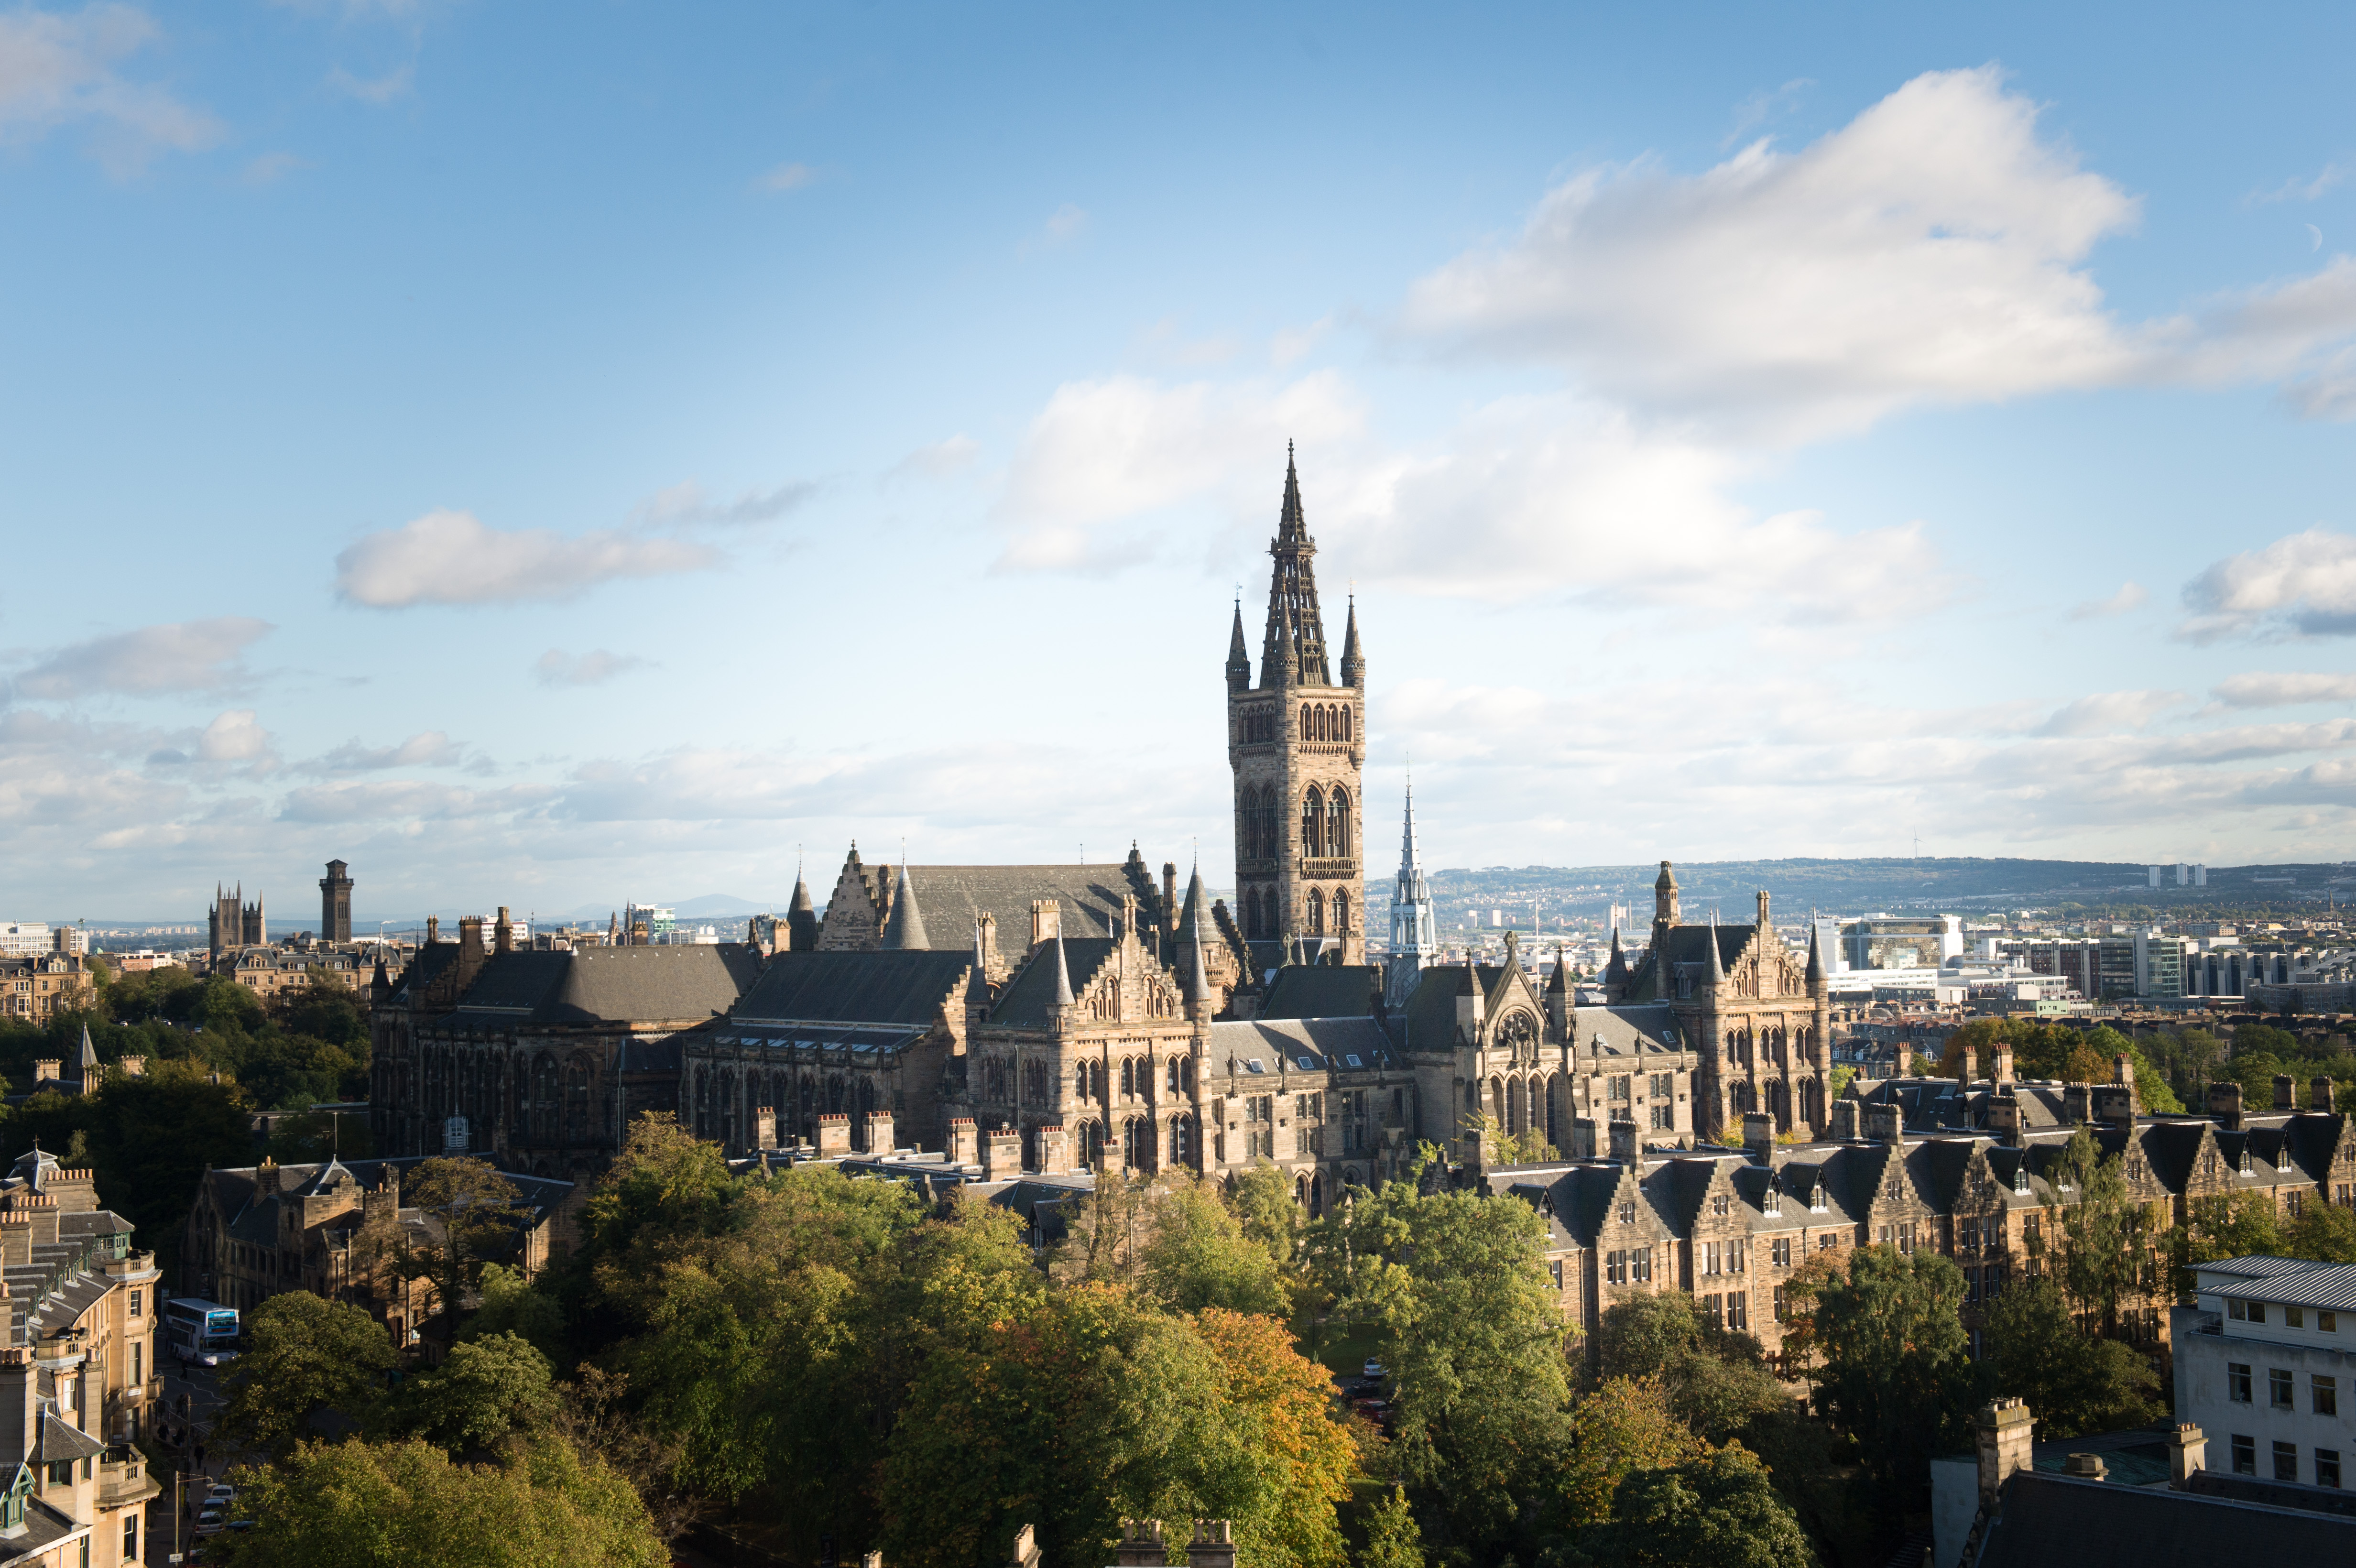
\includegraphics[keepaspectratio=true, height=\paperheight]{../../images/background.jpg}};
    }
    \begin{frame}[plain,noframenumbering]
        \titlepage
    \end{frame}
}

\section{Practical Subgraph-Finding}

\begin{frame}{Subgraph Isomorphism}
    \only<1-2>{
    \centering
    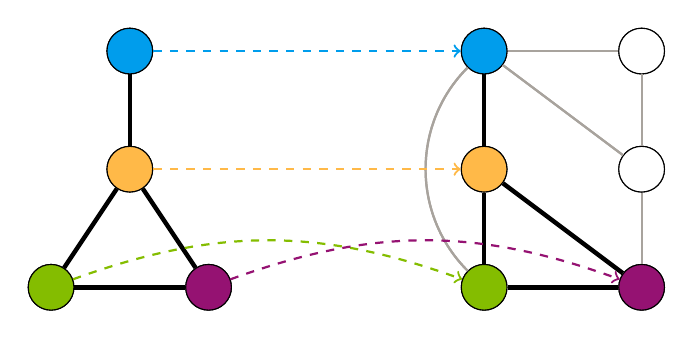
\begin{tikzpicture}
        \node <1> [draw, circle, fill=white, inner sep=4pt, font=\bfseries] (Na) at (1,  0) {\vphantom{1}};
        \node <1> [draw, circle, fill=white, inner sep=4pt, font=\bfseries] (Nb) at (1, -1.5) {\vphantom{1}};
        \node <1> [draw, circle, fill=white, inner sep=4pt, font=\bfseries] (Nc) at (0, -3) {\vphantom{1}};
        \node <1> [draw, circle, fill=white, inner sep=4pt, font=\bfseries] (Nd) at (2, -3) {\vphantom{1}};

        \node <2> [draw, circle, fill=uofgcobalt, inner sep=4pt, font=\bfseries] (Na) at (1,  0) {\vphantom{1}};
        \node <2> [draw, circle, fill=uofgpumpkin, inner sep=4pt, font=\bfseries] (Nb) at (1, -1.5) {\vphantom{1}};
        \node <2> [draw, circle, fill=uofglawn, inner sep=4pt, font=\bfseries] (Nc) at (0, -3) {\vphantom{1}};
        \node <2> [draw, circle, fill=uofgthistle, inner sep=4pt, font=\bfseries] (Nd) at (2, -3) {\vphantom{1}};

        \draw [ultra thick] (Na) -- (Nb);
        \draw [ultra thick] (Nb) -- (Nc);
        \draw [ultra thick] (Nc) -- (Nd);
        \draw [ultra thick] (Nb) -- (Nd);

        \node <1> [draw, circle, fill=white, inner sep=4pt, font=\bfseries] (N1) at (5.5,  0) {\vphantom{1}};
        \node <1> [draw, circle, fill=white, inner sep=4pt, font=\bfseries] (N2) at (7.5,  0) {\vphantom{1}};
        \node <1> [draw, circle, fill=white, inner sep=4pt, font=\bfseries] (N3) at (5.5, -1.5) {\vphantom{1}};
        \node <1> [draw, circle, fill=white, inner sep=4pt, font=\bfseries] (N4) at (7.5, -1.5) {\vphantom{1}};
        \node <1> [draw, circle, fill=white, inner sep=4pt, font=\bfseries] (N5) at (5.5, -3) {\vphantom{1}};
        \node <1> [draw, circle, fill=white, inner sep=4pt, font=\bfseries] (N6) at (7.5, -3) {\vphantom{1}};

        \node <2> [draw, circle, fill=uofgcobalt, inner sep=4pt, font=\bfseries] (N1) at (5.5,  0) {\vphantom{1}};
        \node <2> [draw, circle, fill=white, inner sep=4pt, font=\bfseries] (N2) at (7.5,  0) {\vphantom{1}};
        \node <2> [draw, circle, fill=uofgpumpkin, inner sep=4pt, font=\bfseries] (N3) at (5.5, -1.5) {\vphantom{1}};
        \node <2> [draw, circle, fill=white, inner sep=4pt, font=\bfseries] (N4) at (7.5, -1.5) {\vphantom{1}};
        \node <2> [draw, circle, fill=uofglawn, inner sep=4pt, font=\bfseries] (N5) at (5.5, -3) {\vphantom{1}};
        \node <2> [draw, circle, fill=uofgthistle, inner sep=4pt, font=\bfseries] (N6) at (7.5, -3) {\vphantom{1}};

        \draw <1> [thick, color=uofgsandstone!50] (N1) -- (N2);
        \draw <1> [thick, color=uofgsandstone!50] (N1) -- (N3);
        \draw <1> [thick, color=uofgsandstone!50] (N1) -- (N4);
        \draw <1> [thick, color=uofgsandstone!50] (N2) -- (N4);
        \draw <1> [thick, color=uofgsandstone!50] (N3) -- (N5);
        \draw <1> [thick, color=uofgsandstone!50] (N3) -- (N6);
        \draw <1> [thick, color=uofgsandstone!50] (N4) -- (N6);
        \draw <1> [thick, color=uofgsandstone!50] (N5) -- (N6);
        \draw <1> [thick, color=uofgsandstone!50] (N1) to [in=135, out=225] (N5);

        \draw <2> [thick, color=uofgsandstone!50] (N1) -- (N2);
        \draw <2> [ultra thick] (N1) -- (N3);
        \draw <2> [thick, color=uofgsandstone!50] (N1) -- (N4);
        \draw <2> [thick, color=uofgsandstone!50] (N2) -- (N4);
        \draw <2> [ultra thick] (N3) -- (N5);
        \draw <2> [ultra thick] (N3) -- (N6);
        \draw <2> [thick, color=uofgsandstone!50] (N4) -- (N6);
        \draw <2> [ultra thick] (N5) -- (N6);
        \draw <2> [thick, color=uofgsandstone!50] (N1) to [in=135, out=225] (N5);

        \draw <2> [thick, dashed, color=uofgcobalt, arrows=->] (Na) to (N1);
        \draw <2> [thick, dashed, color=uofgpumpkin, arrows=->] (Nb) to (N3);
        \draw <2> [thick, dashed, color=uofglawn, arrows=->] (Nc) to [out=20, in=160] (N5);
        \draw <2> [thick, dashed, color=uofgthistle, arrows=->] (Nd) to [out=20, in=160] (N6);
    \end{tikzpicture}}

\begin{itemize}
    \item Find the \emph{pattern} inside the \emph{target}.
    \item Applications in compilers, biochemistry, model checking, pattern recognition, \ldots
    \item Often want to find \emph{all} matches.
\end{itemize}
\end{frame}

\begin{frame}{The Maximum Clique Problem}
    \begin{center}
    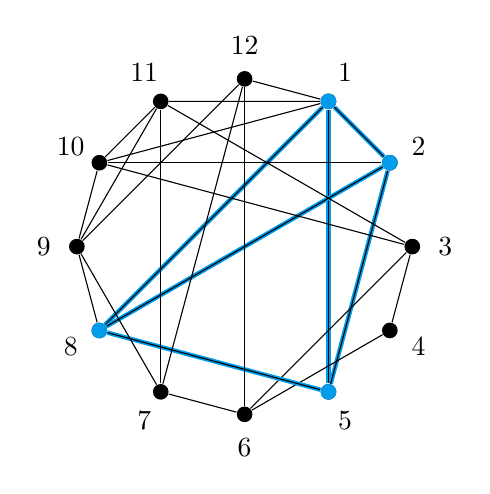
\begin{tikzpicture}
        \begin{scope}[scale=1.5]
        \newcount \myc
        \foreach \n in {3, 4, 6, 7, 9, 10, 11, 12}{
            \myc=\n \advance\myc by -1 \multiply\myc by -360 \divide\myc by 12 \advance\myc by 60.0
            \node[anchor=center] (L\n) at (\the\myc:1.7) {\n};
            \node[anchor=center, circle, fill=black, inner sep=2pt] (N\n) at (\the\myc:1.42) {};
        }
        \foreach \n in {1, 2, 5, 8}{
            \myc=\n \advance\myc by -1 \multiply\myc by -360 \divide\myc by 12 \advance\myc by 60.0
            \node[anchor=center] (L\n) at (\the\myc:1.7) {\n};
            \node<1>[anchor=center, circle, fill=black, inner sep=2pt] (N\n) at (\the\myc:1.42) {};
            \node<2>[anchor=center, circle, fill=uofgcobalt, inner sep=2pt] (N\n) at (\the\myc:1.42) {};
        }
        \draw <2> [ultra thick, color=uofgcobalt] (N1) -- (N2);
        \draw <2> [ultra thick, color=uofgcobalt] (N1) -- (N5);
        \draw <2> [ultra thick, color=uofgcobalt] (N1) -- (N8);
        \draw <1> (N1) -- (N2);
        \draw <1> (N1) -- (N5);
        \draw <1> (N1) -- (N8);
        \draw (N1) -- (N10);
        \draw (N1) -- (N11);
        \draw (N1) -- (N12);
        \draw <2> [ultra thick, color=uofgcobalt] (N2) -- (N5);
        \draw <2> [ultra thick, color=uofgcobalt] (N2) -- (N8);
        \draw <1> (N2) -- (N5);
        \draw <1> (N2) -- (N8);
        \draw (N2) -- (N10);
        \draw (N3) -- (N4);
        \draw (N3) -- (N6);
        \draw (N3) -- (N10);
        \draw (N3) -- (N11);
        \draw (N4) -- (N6);
        \draw <2> [ultra thick, color=uofgcobalt] (N5) -- (N8);
        \draw <1> (N5) -- (N8);
        \draw (N6) -- (N7);
        \draw (N6) -- (N12);
        \draw (N7) -- (N9);
        \draw (N7) -- (N11);
        \draw (N7) -- (N12);
        \draw (N8) -- (N9);
        \draw (N9) -- (N10);
        \draw (N9) -- (N11);
        \draw (N9) -- (N12);
        \draw (N10) -- (N11);
    \end{scope}
    \end{tikzpicture}
\end{center}
\end{frame}

\begin{frame}{Constraint Programming}
    \begin{itemize}
        \item We have a set of \emph{variables}.
        \item Each variable has a finite \emph{domain}.
        \item We have \emph{constraints} between variables.
        \item Give each variable a value from its domain, satisfying all constraints (and maybe
            maximise some objective).
        \item Solve using inference and intelligent backtracking search.
    \end{itemize}
\end{frame}

\begin{frame}{Worst-Case Complexity vs Practice}
    \begin{itemize}
        \item These problems are NP-hard, hard to approximate, etc.
        \item We can solve maximum clique on larger graphs than all-pairs shortest path.
        \item We don't have a deep understanding as to why.
    \end{itemize}
\end{frame}

\begin{frame}{The Slight Problem\ldots}
    \begin{itemize}
        \item State of the art solvers occasionally produce incorrect answers.
        \item <2-> Extensive testing?
            \begin{itemize}
                \item <2-> Only uncovers superficial bugs.
                \item <2-> Empirically unsuccessful, even if people try really hard.
            \end{itemize}
        \item <3-> Formal methods?
            \begin{itemize}
                \item <3-> Far from being able to handle state of the art algorithms and solvers.
            \end{itemize}
    \end{itemize}
\end{frame}

\section{Proof Logging for SAT}

\begin{frame}{Proof Logging}
        \vspace*{-1em}
        \begin{center}
        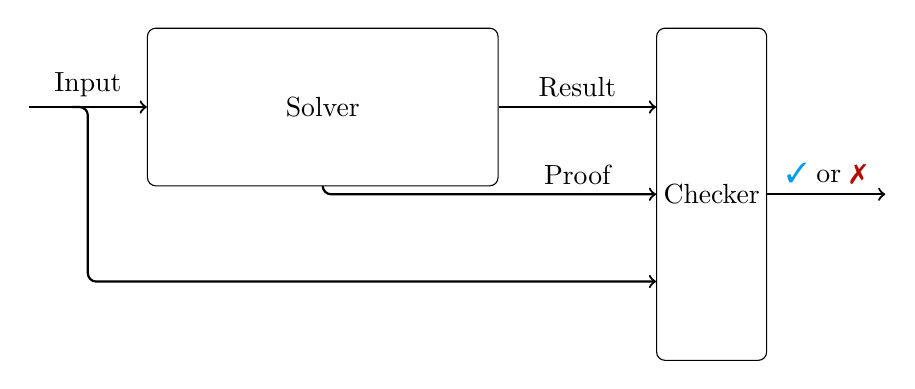
\begin{tikzpicture}
            \node (solver) [%
            inner xsep=5em,
            inner ysep=2.5em, 
            draw, rounded corners=3pt] { Solver };

            \node (checker) [%
            right=2cm of solver.north east, 
            anchor=north west,
            inner xsep=0.25em,
            draw, rounded corners=3pt, 
            minimum height=12em,
            visible on=<3->] { Checker };

            \draw [->, thick] (solver.east) -- (solver.east -| checker.west)
                coordinate [midway] (solutionmid) node [above, midway]
                { Result };

            \draw [->, thick, rounded corners=3pt, visible on=<2->] (solver.south) -- (solver.south |- checker.west)
                -- (checker.west) coordinate [midway] (proofmid);

            \coordinate (prooflabel) at (proofmid-|solutionmid);
            \node [above=0cm of prooflabel, visible on=<2->] { Proof };

            \coordinate [right=1.5cm of checker.east] (verified);
            \draw [->, thick, visible on=<4->] (checker.east) -- (verified) node [above, midway] {
                \textcolor{uofgcobalt}{\ding{51}} or \textcolor{uofgpillarbox}{\ding{55}} };

            \coordinate [left=1.5cm of solver.west] (input);
            \draw [->, thick] (input) -- (solver.west) coordinate [midway] (inputmid) node [above, midway] { Input };

            \coordinate (checkerbotleft) at ($(checker.west)+($(checker.west)-(solver.east-|checker.west)$)$);

            \draw [->, thick, rounded corners=3pt, visible on=<3->] ($(inputmid)+(-0.2,0)$) -- (inputmid) -- (inputmid |- checkerbotleft) -- (checkerbotleft);
        \end{tikzpicture}
      \end{center}

      \vspace{-10mm}

  \begin{enumerate}
  \item<1->
    Run solver on problem input.
  \item<2->
    Get as output not only 
    result   %%%   solution   % -JN
    but also proof.
  \item<3->
    Feed input + 
    result   %%%   solution 
    + proof to proof checker.
  \item<4->
    Verify that proof checker says 
    result   %%%   solution 
    is     correct.
  \end{enumerate}
\end{frame}

\begin{frame}{What Is A Proof?}
    \begin{center}
        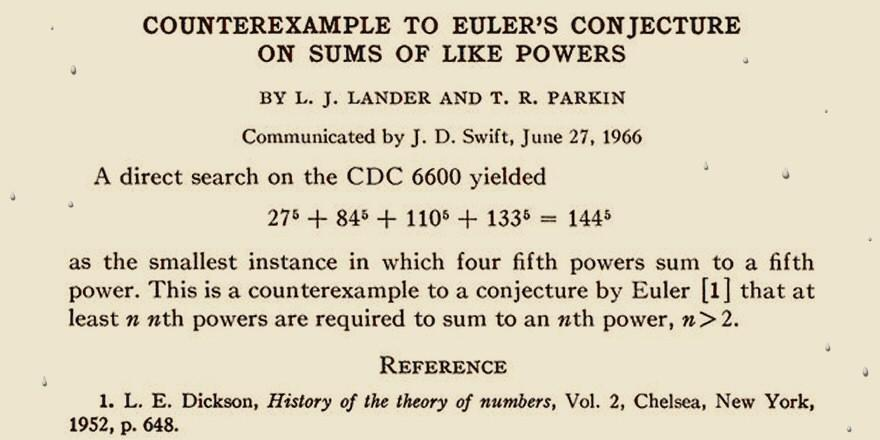
\includegraphics[keepaspectratio=true,scale=0.30]{shortest-math-paper.jpg}
    \end{center}
\end{frame}

\providecommand{\litell}{\ell}
\providecommand{\clwidth}{k}

\begin{frame}
  \frametitle{The SAT Problem}

  \vspace{-1mm}
  
  \begin{itemize}
  \item
    \alertblue{Variable} $\varx$: 
    takes value 
%       $1$ (\textbf{true})
    \textbf{true} ($=\!1$)
    or 
%       $0$ (\textbf{false})
    \textbf{false} ($=\!0$)

    \medskip

  \item
    \alertblue{Literal} 
%       $\lita$:  
    $\litell$:  
    variable 
    $\varx$ or its negation
    $\olnot{\varx}$ 
%       (%which we will 
%       %from now on 
%       write
%       $\olnot{\varx}$ 
%       instead of
%       $\lnot{\varx}$)
    

    \medskip
    
  \item
    \alertblue{Clause}
    $\clc = \litell_1 \lor \cdots \lor \litell_{\clwidth}$:
    disjunction of literals \\
    (Consider 
%    clauses 
    as sets, so
    no repetitions and order 
%        is
    irrelevant)
    
    \medskip
    
  \item
    \alertred{%
      Conjunctive normal form (CNF)
%         CNF 
      formula}
    $\formf = \clc_1 \land \cdots \land \clc_m$:
    conjunction of clauses         
    
%        \bigskip
%        
%      \item
%        \alertred{\kcnfform{}}:  
%        CNF formula with clauses of size $\leq \clwidth$ \\
%        (assume $\clwidth$ fixed)    
%    
%        \bigskip
%        
%      \item
%        Refer to clauses of \cnfform as
%        \introduceterm{axioms} \\
%        (as opposed to derived clauses)
%    
  \end{itemize}
      

%     \pause
%     \bigskip
  \medskip
  
  \begin{block}{The SAT Problem}
    Given a CNF formula~$\formf$, is it satisfiable?
  \end{block}

%     \pause
%     \bigskip
  \medskip
  
  For instance, what about:
  \begingroup
  \small
  \begin{gather*}
%       &
    ( p \lor \overline{u} )
    \land 
    ( q \lor r )
    \land 
    ( \overline{r} \lor w )
    \land
    ( u \lor x \lor y )
      \ \land \
    \\
%%%    
%       \land \
%       &
    ( x \lor \overline{y} \lor z )
    \land
    ( \overline{x} \lor z )
    \land 
    ( \overline{y} \lor \overline{z} )
    \land 
    ( \overline{x} \lor \overline{z} )
    \land
    ( \overline{p} \lor \overline{u} )
  \end{gather*}
  \endgroup
%   
%     For instance, 
%     what about our example formula?
%     \begin{align*}
%       %        F = \ \ \ \ \  
%       &
%       ( x \lor z ) \land
%       ( y \lor \olnot{z} ) \land
%       ( x \lor \olnot{y} \lor u ) \land
%       ( \olnot{y} \lor \olnot{u} ) \\
%       \land \    
%       &( u \lor v ) \land
%       ( \olnot{x} \lor \olnot{v} ) \land
%       ( \olnot{u} \lor w ) \land
%       ( \olnot{x} \lor \olnot{u} \lor \olnot{w} ) 
%     \end{align*}
%   
  
\end{frame}

%%% Local Variables:
%%% mode: latex
%%% TeX-master: "ProofCplxSATsurvey"
%%% End:



\begin{frame}{Proofs for SAT}

    For satisfiable instances: just
%%% THIS IS JUST confusing at this stage... -JN 
%       give (something that propagates to) 
    specify
    a satisfying assignment.
    \\ \medskip
    For unsatisfiability: 
%       a proof is 
    a sequence of clauses (CNF constraints).
    \begin{itemize}
        \item 
          Each clause follows ``obviously'' from everything we know so far.
        \item 
          Final clause is empty, meaning contradiction (written $\bot$).
        \item
          Means original formula must be inconsistent.
    \end{itemize}
\end{frame}

\begin{frame}[t]{What Is Obvious? Unit Propagation}


  \begin{block}{Unit Propagation}
    Clause
    $\clc$
    \colorblue{unit propagates}
    $\litell$ under partial assignment $\rho$
    if
    $\rho$ falsifies all literals in
    $\clc$ except~$\litell$.
  \end{block}

  \pause
  \bigskip

  \textbf{Example:} Unit propagate for
  $\rho = \set{ p \mapsto 0, q\mapsto 0}$ on
%   
%     \vspace{-4mm}
%   
  \begingroup
  \footnotesize
  \begin{equation*}%
    \cdclformulaleftadjust
    ( 
    \alertred<3->{p} \lor 
    \alertblue<4->{\overline{u}}
    )
    \landwsp 
    ( \alertred<3->{q}
    \lor
    \alertblue<5->{r} 
    )
    \landwsp 
    (
    \alertred<5->{\overline{r}}
    \lor 
    \alertblue<6->{w} 
    )
    \landwsp
    ( 
    \alertred<4->{u}
    \lor x \lor y )
    \landwsp
    ( x \lor \overline{y} \lor z )
    \landwsp 
    ( \overline{x} \lor z )
    \landwsp 
    ( \overline{y} \lor \overline{z} )
    \landwsp 
    ( \overline{x} \lor \overline{z} )
    \landwsp
    ( 
    \alertblue<3->{\overline{p}} 
    \lor
    \alertblue<4->{\overline{u}}
    )
  \end{equation*}
  \endgroup

  \vspace{-2mm}
 
  \begin{itemize}
  \item<4-> 
    $p \lor \overline{u}$ propagates $u \mapsto 0$.

  \item<5-> 
    $q \lor r$ propagates $r \mapsto 1$.

  \item<6-> 
    Then
    $\overline{r} \lor w$ propagates $w \mapsto 1$.

  \item<7-> 
    No further unit propagations.
  \end{itemize}

  \medskip

  \uncover<8->{%
    Proof checker should 
%       be smart enough to 
    know how to
    unit propagate until saturation.
  }

\end{frame}

\begin{frame}[t]%
%     {Forward Checking (DPLL)}
  {Davis-Putman-Logemann-Loveland (DPLL)}

    DPLL:
  Assign variables and propagate;
  backtrack when clause violated.

  \medskip

%%%   
%%% Lots of text... Try to be more concise -JN  
%%%   
%     We could write a ``proof'' of unsatisfiability
%     by writing a step whenever a forward-checker backtracks
%     asserting the negation of the guesses we made. For example,
%     

  ``Proof trace'':
  when backtracking, write negation
  of guesses made. 


%%%%%
%%%%% Changed to an example that is simpler when highlighting is added -JN
%%%%%

  \begingroup
  \footnotesize
  \begin{equation*}%
%%%
%%% FORMULA *WITH* HIGHLIGHTING
%%%
    \cdclformulaleftadjust
    ( 
    \alertblue<5-5>{p}
    \lor 
    \alertred<4-5>{\overline{u}}
    )
    \landwsp 
    ( 
    q 
    \lor 
    r 
    )
    \landwsp 
    ( 
    \overline{r} 
    \lor
    w 
    )
    \landwsp
    ( 
    \alertblue<4-5>{u} 
    \lor 
    \only<1-8>{\alertred<2-8>{x}} 
    \only<9->{\alertblue<9-10>{x}} 
    \lor 
    \only<1-5>{\alertred<3-5>{y}} 
    \only<6->{\alertblue<6-7>{y}} 
    )
    \landwsp
    ( 
    \only<1-8>{\alertred<2-8>{x}}
    \only<9->{\alertblue<9-10>{x}}  
    \lor 
    \only<1-5>{\alertblue<3-5>{\overline{y}}}
    \only<6->{\alertred<6-7>{\overline{y}}} 
    \lor 
    \alertblue<7,10>{z} 
    )
    \landwsp 
    ( 
    \only<1-8>{\alertblue<2-8>{\overline{x}}}
    \only<9->{\alertred<9-10>{\overline{x}}}  
    \lor 
    \alertblue<7,10>{z} 
    )
    \landwsp 
    ( 
    \only<1-5>{\alertblue<3-5>{\overline{y}}}
    \only<6->{\alertred<6-7>{\overline{y}}} 
    \alertred<7>{\lor}
    \alertred<7,10>{\overline{z}}
    )
    \landwsp 
    ( 
    \only<1-8>{\alertblue<2-8>{\overline{x}}}
    \only<9->{\alertred<9-10>{\overline{x}}}  
    \alertred<10>{\lor} 
    \alertred<7,10>{\overline{z}}
    )
    \landwsp
    (
    \alertred<5-5>{\overline{p}}
    \alertred<5-5>{\lor} 
    \alertred<4-5>{\overline{u}}
    )
%%%
%%% FORMULA WITHOUT HIGHLIGHTING
%%%
%       \cdclformulaleftadjust
%       ( p \lor \overline{u} )
%       \landwsp 
%       ( q \lor r )
%       \landwsp 
%       ( \overline{r} \lor w )
%       \landwsp
%       ( u \lor x \lor y )
%       \landwsp
%       ( x \lor \overline{y} \lor z )
%       \landwsp 
%       ( \overline{x} \lor z )
%       \landwsp 
%       ( \overline{y} \lor \overline{z} )
%       \landwsp 
%       ( \overline{x} \lor \overline{z} )
%       \landwsp
%       ( \overline{p} \lor \overline{u} )
  \end{equation*}
  \endgroup
  
  \bigskip
  
  \begin{columns}[T]%
    \begin{column}{0.4\textwidth}
      \begin{enumerate}
      \item <5-> $x \lor y$
      \item <7-> $x \lor \olnot{y}$
      \item <8-> $x$
      \item <10-> $\olnot{x}$
      \item <11-> $\emptycl$
      \end{enumerate}
    \end{column}
    \begin{column}{0.5\textwidth}
%%%
%%% SEARCH TREE *WITH* OVERLAYS FOR HIGHLIGHTING
%%%
      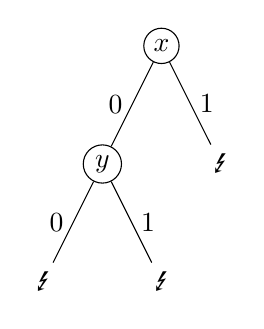
\begin{tikzpicture}<2->%
        [sibling distance=4em, level distance=3.5em, align=center]
        \node [draw, circle, inner sep=2pt, visible on=<2->] {$x$}
        child { node [draw, circle, inner sep=2pt, visible on=<3->] {$y$}
          child { node [visible on=<5->] {\Lightning} edge from parent [visible on=<3->] node [left, visible on=<3->] { 
$0$  %  $\overline{y}$ 
} }
          child { node [visible on=<7->] {\Lightning} edge from parent [visible on=<6->] node [right, visible on=<6->] { 
$1$ % $y$ 
} }
          edge from parent [visible on=<2->] node [left, visible on=<2->] { 
$0$ % $\overline{x}$ 
}
        }
        child { node [visible on=<10->] {\Lightning}
          edge from parent [visible on=<9->] node [right, visible on=<9->] { 
$1$  % $x$
 }
        }
        ;
      \end{tikzpicture}
    \end{column}
  \end{columns}
\end{frame}

\begin{frame}{Reverse Unit Propagation (RUP)}

  To make this a proof, need 
%       each backtrack clause  %%% Trying to fit on one line -JN
  backtrack clauses 
  to be easily verifiable.

  \pause
  
  \begin{block}{Reverse unit propagation (RUP) clause}
    $\clc$ is a 
    \colorblue{reverse unit propagation (RUP)} 
    clause \wrt $\formf$ if
    \begin{itemize}
    \item 
      assigning $\clc$ to false,
    \item 
      then unit propagating on $\formf$ until saturation
    \item 
      leads to contradiction
    \end{itemize}
    If so, 
    $\formf$ clearly  implies  $\clc$,
    and condition easy to verify efficiently
  \end{block}

  \pause
  
  \begin{block}{Fact}
%       Backtracks 
    Backtrack clauses
    from DPLL solver generate a RUP proof.
  \end{block}

\end{frame}

\begin{frame}{RUP Proofs and CDCL}
\begin{block}{Fact}
  All learned clauses generated by CDCL solver are RUP clauses.
\end{block}

\pause
\bigskip

  So short proof of unsatisfiability for
  \begingroup
  \footnotesize
  \begin{equation*}%
    \cdclformulaleftadjust
    (
    \alertblue<11>{p} 
    \lor 
    \alertblue<3-5>{\alertred<10-11>{\overline{u}}} 
    ) 
    \landwsp
    {( q \lor r )}
    \landwsp
    {( \overline{r} \lor w )}
    \landwsp
    (
    \alertblue<10-11>{\alertred<3-5>{u}} 
    \lor  
    \alertblue<6-7>{\alertred<3-5,9-11>{x}} 
    \lor 
    \alertblue<4-5>{y} 
    )
    \landwsp
    ( 
    \alertblue<6-7>{\alertred<3-5,9-11>{x}} 
    \lor 
    \alertred<4-5>{\overline{y}} 
    \lor 
    \alertblue<5,7>{z}
    )  
    \landwsp
    (
    \alertblue<3-5,9-11>{\alertred<6-7>{\overline{x}}}
    \lor
    \alertblue<5,7>{z} 
    )
    \landwsp
    (
    \alertred<4-5>{\overline{y}} 
    \alertred<5>{\lor} 
    \alertred<5,7>{\overline{z}}
    ) 
    \landwsp
    (
    \alertblue<3-5,9-11>{\alertred<6-7>{\overline{x}}}
    \alertred<7>{\lor} 
    \alertred<5,7>{\overline{z}} 
    )
    \landwsp
    (
    \alertred<11>{\overline{p}} 
    \alertred<11>{\lor}
    \alertblue<3-5>{\alertred<10-11>{\overline{u}}} 
    )
  \end{equation*}
  \endgroup
  % 
  is sequence of 
  reverse unit propagation (RUP)
  clauses
  \begin{enumerate}
  \item 
    \alertred<3-5>{$\alertblue<10-11>{u} \lor
      \alertblue<6-7>{\alertred<9-11>{x}}$}
  \item 
    \alertred<6-7>{\alertblue<9-11>{$\olnot{x}$}}
  \item 
      \alertred<8-11>{$\emptycl$}
  \end{enumerate}
\end{frame}

\begin{frame}{Resolution Proofs}
    \begin{block}{Fact}
        RUP proofs can be seen as shorthand for Resolution proofs.
    \end{block}

    \bigskip

    \begin{minipage}[c]{0.25\framewidth}
        \textcolor{uofgcobalt}{\textbf{Model axioms}}
    \end{minipage}\hfill\begin{minipage}[c]{0.70\framewidth}
        \centering From the input
    \end{minipage}\bigskip

    \begin{minipage}[c]{0.25\framewidth}
        \textcolor{uofgcobalt}{\textbf{Resolution}}
    \end{minipage}\hfill\begin{minipage}[c]{0.70\framewidth}\begin{prooftree}
        \AxiomC{$\textcolor{uofglawn}{x_1} \vee \textcolor{uofglawn}{x_2} \vee \ldots \vee
        \textcolor{uofglawn}{x_i} \vee \textcolor{uofgpillarbox}{c}$}
        \AxiomC{$\textcolor{uofgpillarbox}{\overline{c}} \vee \textcolor{uofgcobalt}{y_1} \vee
        \textcolor{uofgcobalt}{y_2} \vee \ldots \textcolor{uofgcobalt}{y_j}$}
        \BinaryInfC{$\textcolor{uofglawn}{x_1} \vee \textcolor{uofglawn}{x_2} \vee \ldots \vee
        \textcolor{uofglawn}{x_i} \vee \textcolor{uofgcobalt}{y_1} \vee
        \textcolor{uofgcobalt}{y_2} \vee \ldots \vee \textcolor{uofgcobalt}{y_j}$}
    \end{prooftree}\end{minipage}

    \bigskip

    \begin{itemize}
        \item To prove unsatisfiability: resolve until you reach the empty clause.
    \end{itemize}
\end{frame}

\section{Beyond SAT}

\begin{frame}{Resolution Can't Count}
    \begin{itemize}
        \item In subgraph isomorphism, can't map a pattern vertex with $n$ vertices
            into a target graph with $n - 1$ vertices.
        \item This requires exponential length proofs in resolution!
    \end{itemize}
\end{frame}

\begin{frame}{From CNF to Pseudo-Boolean}
    \begin{itemize}
        \item A set of $\{ 0, 1 \}$-valued variables $x_i$, $1$ means true.
        \item Constraints are linear inequalities \[
                \sum_i c_i x_i \ge C
            \]
        \item Write $\overline{x}_i$ to mean $1 - x_i$.
        \item Can rewrite CNF to pseudo-Boolean directly, \begin{align*}
                & x_1 \vee \overline{x}_2 \vee x_3 & \leftrightarrow && x_1 + \overline{x}_2 + x_3 \ge 1
        \end{align*}
    \end{itemize}
\end{frame}

\begin{frame}{Cutting Planes Proofs}
    \begin{minipage}[c]{0.35\framewidth}
        \textcolor{uofgcobalt}{\textbf{Model axioms}}
    \end{minipage}\hfill\begin{minipage}[c]{0.60\framewidth}
        \centering From the input
    \end{minipage}\bigskip

    \begin{minipage}[c]{0.35\framewidth}
        \textcolor{uofgcobalt}{\textbf{Literal axioms}}
    \end{minipage}\hfill\begin{minipage}[c]{0.60\framewidth}\begin{prooftree}
        \AxiomC{~}
        \UnaryInfC{$\ell_i \ge 0$}
    \end{prooftree}\end{minipage}\bigskip

    \begin{minipage}[c]{0.35\framewidth}
        \textcolor{uofgcobalt}{\textbf{Addition}}
    \end{minipage}\hfill\begin{minipage}[c]{0.60\framewidth}\begin{prooftree}
        \AxiomC{$\sum_i a_i \ell_i \ge A$}
        \AxiomC{$\sum_i b_i \ell_i \ge B$}
        \BinaryInfC{$\sum_i (a_i + b_i) \ell_i \ge A + B$}
    \end{prooftree}\end{minipage}\bigskip

    \begin{minipage}[c]{0.35\framewidth}
        \textcolor{uofgcobalt}{\textbf{Multiplication}}\\
        for any $c \in \mathbb{N^+}$
    \end{minipage}\hfill\begin{minipage}[c]{0.60\framewidth}\begin{prooftree}
        \AxiomC{$\sum_i a_i \ell_i \ge A$}
        \UnaryInfC{$\sum_i { c a_i \ell_i } \ge c A$}
    \end{prooftree}\end{minipage}\bigskip

    \begin{minipage}[c]{0.35\framewidth}
        \textcolor{uofgcobalt}{\textbf{Division}}\\
        for any $c \in \mathbb{N^+}$
    \end{minipage}\hfill\begin{minipage}[c]{0.60\framewidth}\begin{prooftree}
        \AxiomC{$\sum_i a_i \ell_i \ge A$}
        \UnaryInfC{$\sum_i {\left\lceil \frac{a_i}{c} \right\rceil} \ell_i \ge \left\lceil \frac{A}{c} \right\rceil$}
    \end{prooftree}\end{minipage}\bigskip
\end{frame}

\begin{frame}{Interleaving RUP and Cutting Planes}
    \begin{itemize}
        \item Can define RUP similarly for pseudo-Boolean constraints.
        \item It does the same thing on clauses.
        \item Idea: use RUP for backtracking, and include explicit cutting
            planes steps to justify reasoning.
    \end{itemize}
\end{frame}

\begin{frame}{The VeriPB System}
    \begin{center}
        \url{https://gitlab.com/MIAOresearch/software/VeriPB} \\
        \bigskip
    \end{center}
    \begin{itemize}
        \item MIT licence, written in Python with parsing in C++.
        \item Useful features like tracing and proof debugging.
    \end{itemize}
\end{frame}

\begin{frame}{Making a Proof-Logging Clique Solver}
    \begin{enumerate}
        \item Output a pseudo-Boolean encoding of the problem.
            \begin{itemize}
                \item Clique problems have several standard file formats.
            \end{itemize}
        \item Make the solver log its search tree.
            \begin{itemize}
                \item Output a small header.
                \item Output something on every backtrack.
                \item Output something every time a solution is found.
                \item Output a small footer.
            \end{itemize}
        \item Figure out how to log the bound function.
    \end{enumerate}
\end{frame}

\begin{frame}{A Slightly Different Workflow}
    \begin{center}
        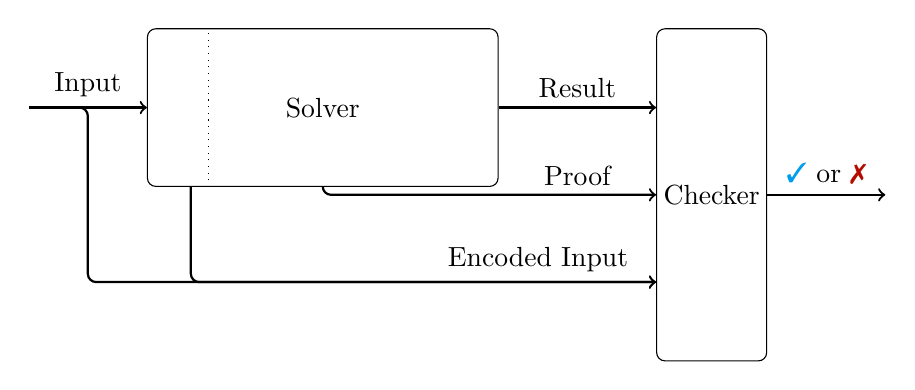
\begin{tikzpicture}
            \node (solver) [inner xsep=5em, inner ysep=2.5em, draw, rounded corners=3pt] { Solver };

            \node (checker) [right=2cm of solver.north east, anchor=north west,
            inner xsep=0.25em, draw, rounded corners=3pt, minimum height=12em, visible on=<3->] { Checker };

            \draw [->, thick] (solver.east) -- (solver.east -| checker.west)
                coordinate [midway] (solutionmid) node [above, midway] { Result };

            \draw [->, thick, rounded corners=3pt, visible on=<2->] (solver.south) -- (solver.south |- checker.west)
                -- (checker.west) coordinate [midway] (proofmid);

            \coordinate (prooflabel) at (proofmid-|solutionmid);
            \node [above=0cm of prooflabel, visible on=<2->] { Proof };

            \coordinate [right=1.5cm of checker.east] (verified);
            \draw [->, thick, visible on=<5->] (checker.east) -- (verified) node [above, midway] {
                \textcolor{uofgcobalt}{\ding{51}} or \colorred{\ding{55}} };

            \coordinate [left=1.5cm of solver.west] (input);
            \draw [->, thick] (input) -- (solver.west) coordinate [midway] (inputmid) node [above, midway] { Input };

            \coordinate (checkerbotleft) at ($(checker.west)+($(checker.west)-(solver.east-|checker.west)$)$);

            \draw [->, thick, rounded corners=3pt, visible on=<3>] ($(inputmid)+(-0.2,0)$) --
            (inputmid) -- (inputmid |- checkerbotleft) -- (checkerbotleft) coordinate [midway] (altinputmid);
            \coordinate (solverstart) at ($(solver.south)!0.75!(solver.south west)$);
            \coordinate (solverstart2) at ($(solver.south)!0.65!(solver.south west)$);
            \draw [dotted, visible on=<4->] (solverstart2) -- (solverstart2 |- solver.north);
            \draw [->, thick, rounded corners=3pt, visible on=<4->] (solverstart) -- (solverstart |- checkerbotleft) -- (checkerbotleft);

            \coordinate (prooflabel) at (altinputmid-|solutionmid);
            \node [above=0cm of prooflabel, xshift=-0.5cm, visible on=<4->] { Encoded Input };
        \end{tikzpicture}
    \end{center}
\end{frame}

\begin{frame}[fragile]{A Pseudo-Boolean Encoding for Clique (in OPB Format)}
    \begin{center}
    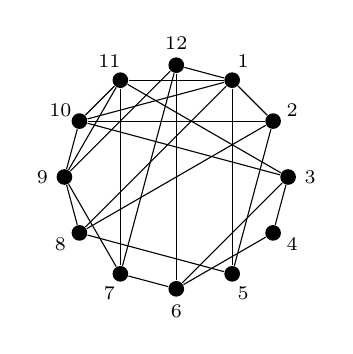
\begin{tikzpicture}
        \begin{scope}[every node/.style = {font=\scriptsize}]
        \newcount \myc
        \foreach \n in {3, 4, 6, 7, 9, 10, 11, 12}{
            \myc=\n \advance\myc by -1 \multiply\myc by -360 \divide\myc by 12 \advance\myc by 60.0
            \node[anchor=center] (L\n) at (\the\myc:1.7) {\n};
            \node[anchor=center, circle, fill=black, inner sep=2pt] (N\n) at (\the\myc:1.42) {};
        }
        \foreach \n in {1, 2, 5, 8}{
            \myc=\n \advance\myc by -1 \multiply\myc by -360 \divide\myc by 12 \advance\myc by 60.0
            \node[anchor=center] (L\n) at (\the\myc:1.7) {\n};
            \node[anchor=center, circle, fill=black, inner sep=2pt] (N\n) at (\the\myc:1.42) {};
        }
            \draw  (N1) -- (N2);
            \draw  (N1) -- (N5);
            \draw  (N1) -- (N8);
        \draw (N1) -- (N10);
        \draw (N1) -- (N11);
        \draw (N1) -- (N12);
            \draw  (N2) -- (N5);
            \draw  (N2) -- (N8);
        \draw (N2) -- (N10);
        \draw (N3) -- (N4);
        \draw (N3) -- (N6);
        \draw (N3) -- (N10);
        \draw (N3) -- (N11);
        \draw (N4) -- (N6);
            \draw  (N5) -- (N8);
        \draw (N6) -- (N7);
        \draw (N6) -- (N12);
        \draw (N7) -- (N9);
        \draw (N7) -- (N11);
        \draw (N7) -- (N12);
        \draw (N8) -- (N9);
        \draw (N9) -- (N10);
        \draw (N9) -- (N11);
        \draw (N9) -- (N12);
        \draw (N10) -- (N11);
    \end{scope}
    \end{tikzpicture}
\end{center}

\small\begin{Verbatim}[commandchars=\\\{\},codes={\catcode`$=3\catcode`^=7}]
\colorblue{* #variable= 12 #constraint= 41}
min: -1 x1 -1 x2 -1 x3 -1 x4 \emph{\ldots{}and so on\ldots{}} -1 x11 -1 x12 ;
1 ~x3 1 ~x1 >= 1 ;
1 ~x3 1 ~x2 >= 1 ;
1 ~x4 1 ~x1 >= 1 ;
\colorblue{* \ldots{}and a further 38 similar lines for the remaining non-edges}
\end{Verbatim}
\end{frame}

\begin{frame}[fragile,t]{First Attempt at a Proof}%
\only<2>{
\begin{tikzpicture}[overlay,remember picture] \coordinate (header1space) at ($(pic cs:header1)+(0pt,6pt)$); \node[rounded corners, fit = (header1space) (pic cs:header2) (pic cs:header3), fill=uofgsunshine] {};\end{tikzpicture}}%
\only<3>{
\begin{tikzpicture}[overlay,remember picture] \coordinate (opt1space) at ($(pic cs:opt1a)+(0pt,6pt)$); \node[rounded corners, fit = (opt1space) (pic cs:opt1b), fill=uofgsunshine] {};\end{tikzpicture}}%
\only<4>{
\begin{tikzpicture}[overlay,remember picture] \coordinate (bt1space) at ($(pic cs:bt1a)+(0pt,6pt)$); \node[rounded corners, fit = (bt1space) (pic cs:bt1b), fill=uofgsunshine] {};\end{tikzpicture}}%
\only<5>{
\begin{tikzpicture}[overlay,remember picture] \coordinate (bt2space) at ($(pic cs:bt2a)+(0pt,6pt)$); \node[rounded corners, fit = (bt2space) (pic cs:bt2b), fill=uofgsunshine] {};\end{tikzpicture}}%
\only<6>{
\begin{tikzpicture}[overlay,remember picture] \coordinate (bt3space) at ($(pic cs:bt3a)+(0pt,6pt)$); \node[rounded corners, fit = (bt3space) (pic cs:bt3b), fill=uofgsunshine] {};\end{tikzpicture}}%
\only<7>{
\begin{tikzpicture}[overlay,remember picture] \coordinate (bt4space) at ($(pic cs:bt4a)+(0pt,6pt)$); \node[rounded corners, fit = (bt4space) (pic cs:bt4b), fill=uofgsunshine] {};\end{tikzpicture}}%
\only<8>{
\begin{tikzpicture}[overlay,remember picture] \coordinate (opt2space) at ($(pic cs:opt2a)+(0pt,6pt)$); \node[rounded corners, fit = (opt2space) (pic cs:opt2b), fill=uofgsunshine] {};\end{tikzpicture}}%
\only<9>{
\begin{tikzpicture}[overlay,remember picture] \coordinate (bt5space) at ($(pic cs:bt5a)+(0pt,6pt)$); \node[rounded corners, fit = (bt5space) (pic cs:bt5b), fill=uofgsunshine] {};\end{tikzpicture}}%
\only<10>{
\begin{tikzpicture}[overlay,remember picture] \coordinate (bt6space) at ($(pic cs:bt6a)+(0pt,6pt)$); \node[rounded corners, fit = (bt6space) (pic cs:bt6b), fill=uofgsunshine] {};\end{tikzpicture}}%
\only<11>{
\begin{tikzpicture}[overlay,remember picture] \coordinate (bt7space) at ($(pic cs:bt7a)+(0pt,6pt)$); \node[rounded corners, fit = (bt7space) (pic cs:bt7b), fill=uofgsunshine] {};\end{tikzpicture}}%
\only<12>{
\begin{tikzpicture}[overlay,remember picture] \coordinate (contaspace) at ($(pic cs:conta)+(0pt,6pt)$); \node[rounded corners, fit = (contaspace) (pic cs:contb), fill=uofgsunshine] {};\end{tikzpicture}}%
\begin{tikzpicture}[overlay,remember picture]
    \node [xshift=-3cm, yshift=0.5cm] at (current page.east) {
        \begin{tikzpicture}
    \begin{scope}[every node/.style = {font=\scriptsize}]

        \myc=1 \advance\myc by -1 \multiply\myc by -360 \divide\myc by 12 \advance\myc by 60.0
        \node[anchor=center] (L1) at (\the\myc:1.7) {1};
        \node<1-2>[anchor=center, circle, fill=black, inner sep=2pt] (N1) at (\the\myc:1.42) {};
        \node<3>[anchor=center, circle, fill=black!20, inner sep=2pt] (N1) at (\the\myc:1.42) {};
        \node<4>[anchor=center, circle, fill=black!20, inner sep=2pt] (N1) at (\the\myc:1.42) {};
        \node<5>[anchor=center, circle, fill=black, inner sep=2pt] (N1) at (\the\myc:1.42) {};
        \node<6-7>[anchor=center, circle, fill=black, inner sep=2pt] (N1) at (\the\myc:1.42) {};
        \node<8>[anchor=center, circle, fill=uofgcobalt, inner sep=2pt] (N1) at (\the\myc:1.42) {};
        \node<9->[anchor=center, circle, fill=black, inner sep=2pt] (N1) at (\the\myc:1.42) {};

        \myc=2 \advance\myc by -1 \multiply\myc by -360 \divide\myc by 12 \advance\myc by 60.0
        \node[anchor=center] (L2) at (\the\myc:1.7) {2};
        \node<1-2>[anchor=center, circle, fill=black, inner sep=2pt] (N2) at (\the\myc:1.42) {};
        \node<3-7>[anchor=center, circle, fill=black!20, inner sep=2pt] (N2) at (\the\myc:1.42) {};
        \node<8>[anchor=center, circle, fill=uofgcobalt, inner sep=2pt] (N2) at (\the\myc:1.42) {};
        \node<9->[anchor=center, circle, fill=black, inner sep=2pt] (N2) at (\the\myc:1.42) {};

        \myc=3 \advance\myc by -1 \multiply\myc by -360 \divide\myc by 12 \advance\myc by 60.0
        \node[anchor=center] (L3) at (\the\myc:1.7) {3};
        \node<1-2>[anchor=center, circle, fill=black, inner sep=2pt] (N3) at (\the\myc:1.42) {};
        \node<3>[anchor=center, circle, fill=black!20, inner sep=2pt] (N3) at (\the\myc:1.42) {};
        \node<4>[anchor=center, circle, fill=black!20, inner sep=2pt] (N3) at (\the\myc:1.42) {};
        \node<5>[anchor=center, circle, fill=black!20, inner sep=2pt] (N3) at (\the\myc:1.42) {};
        \node<6-7>[anchor=center, circle, fill=black, inner sep=2pt] (N3) at (\the\myc:1.42) {};
        \node<8-10>[anchor=center, circle, fill=black!20, inner sep=2pt] (N3) at (\the\myc:1.42) {};
        \node<11->[anchor=center, circle, fill=black, inner sep=2pt] (N3) at (\the\myc:1.42) {};

        \myc=4 \advance\myc by -1 \multiply\myc by -360 \divide\myc by 12 \advance\myc by 60.0
        \node[anchor=center] (L4) at (\the\myc:1.7) {4};
        \node<1-2>[anchor=center, circle, fill=black, inner sep=2pt] (N4) at (\the\myc:1.42) {};
        \node<3-10>[anchor=center, circle, fill=black!20, inner sep=2pt] (N4) at (\the\myc:1.42) {};
        \node<11->[anchor=center, circle, fill=black, inner sep=2pt] (N4) at (\the\myc:1.42) {};

        \myc=5 \advance\myc by -1 \multiply\myc by -360 \divide\myc by 12 \advance\myc by 60.0
        \node[anchor=center] (L5) at (\the\myc:1.7) {5};
        \node<1-2>[anchor=center, circle, fill=black, inner sep=2pt] (N5) at (\the\myc:1.42) {};
        \node<3-7>[anchor=center, circle, fill=black!20, inner sep=2pt] (N5) at (\the\myc:1.42) {};
        \node<8>[anchor=center, circle, fill=uofgcobalt, inner sep=2pt] (N5) at (\the\myc:1.42) {};
        \node<9>[anchor=center, circle, fill=uofgthistle, inner sep=2pt] (N5) at (\the\myc:1.42) {};
        \node<10>[anchor=center, circle, fill=black!20, inner sep=2pt] (N5) at (\the\myc:1.42) {};
        \node<11->[anchor=center, circle, fill=black, inner sep=2pt] (N5) at (\the\myc:1.42) {};

        \myc=6 \advance\myc by -1 \multiply\myc by -360 \divide\myc by 12 \advance\myc by 60.0
        \node[anchor=center] (L6) at (\the\myc:1.7) {6};
        \node<1-2>[anchor=center, circle, fill=black, inner sep=2pt] (N6) at (\the\myc:1.42) {};
        \node<3>[anchor=center, circle, fill=black!20, inner sep=2pt] (N6) at (\the\myc:1.42) {};
        \node<4-5>[anchor=center, circle, fill=black, inner sep=2pt] (N6) at (\the\myc:1.42) {};
        \node<6-10>[anchor=center, circle, fill=black!20, inner sep=2pt] (N6) at (\the\myc:1.42) {};
        \node<11->[anchor=center, circle, fill=black, inner sep=2pt] (N6) at (\the\myc:1.42) {};

        \myc=7 \advance\myc by -1 \multiply\myc by -360 \divide\myc by 12 \advance\myc by 60.0
        \node[anchor=center] (L7) at (\the\myc:1.7) {7};
        \node<1-2>[anchor=center, circle, fill=black, inner sep=2pt] (N7) at (\the\myc:1.42) {};
        \node<3>[anchor=center, circle, fill=uofgcobalt, inner sep=2pt] (N7) at (\the\myc:1.42) {};
        \node<4>[anchor=center, circle, fill=uofgthistle, inner sep=2pt] (N7) at (\the\myc:1.42) {};
        \node<5-6>[anchor=center, circle, fill=black!20, inner sep=2pt] (N7) at (\the\myc:1.42) {};
        \node<7>[anchor=center, circle, fill=black, inner sep=2pt] (N7) at (\the\myc:1.42) {};
        \node<8-10>[anchor=center, circle, fill=black!20, inner sep=2pt] (N7) at (\the\myc:1.42) {};
        \node<11->[anchor=center, circle, fill=black, inner sep=2pt] (N7) at (\the\myc:1.42) {};

        \myc=8 \advance\myc by -1 \multiply\myc by -360 \divide\myc by 12 \advance\myc by 60.0
        \node<1-10>[anchor=center] (L8) at (\the\myc:1.7) {8};
        \node<11->[anchor=center] (L8) at (\the\myc:1.7) {\phantom{8}};
        \node<1-2>[anchor=center, circle, fill=black, inner sep=2pt] (N8) at (\the\myc:1.42) {};
        \node<3-7>[anchor=center, circle, fill=black!20, inner sep=2pt] (N8) at (\the\myc:1.42) {};
        \node<8>[anchor=center, circle, fill=uofgcobalt, inner sep=2pt] (N8) at (\the\myc:1.42) {};
        \node<9-10>[anchor=center, circle, fill=uofgthistle, inner sep=2pt] (N8) at (\the\myc:1.42) {};

        \myc=9 \advance\myc by -1 \multiply\myc by -360 \divide\myc by 12 \advance\myc by 60.0
        \node[anchor=center] (L9) at (\the\myc:1.7) {9};
        \node<1-2>[anchor=center, circle, fill=black, inner sep=2pt] (N9) at (\the\myc:1.42) {};
        \node<3>[anchor=center, circle, fill=uofgcobalt, inner sep=2pt] (N9) at (\the\myc:1.42) {};
        \node<4>[anchor=center, circle, fill=black, inner sep=2pt] (N9) at (\the\myc:1.42) {};
        \node<5>[anchor=center, circle, fill=black, inner sep=2pt] (N9) at (\the\myc:1.42) {};
        \node<6-7>[anchor=center, circle, fill=black, inner sep=2pt] (N9) at (\the\myc:1.42) {};
        \node<8-9>[anchor=center, circle, fill=black!20, inner sep=2pt] (N9) at (\the\myc:1.42) {};
        \node<10->[anchor=center, circle, fill=black, inner sep=2pt] (N9) at (\the\myc:1.42) {};

        \myc=10 \advance\myc by -1 \multiply\myc by -360 \divide\myc by 12 \advance\myc by 60.0
        \node[anchor=center] (L10) at (\the\myc:1.7) {10};
        \node<1-2>[anchor=center, circle, fill=black, inner sep=2pt] (N10) at (\the\myc:1.42) {};
        \node<3>[anchor=center, circle, fill=black!20, inner sep=2pt] (N10) at (\the\myc:1.42) {};
        \node<4>[anchor=center, circle, fill=black!20, inner sep=2pt] (N10) at (\the\myc:1.42) {};
        \node<5>[anchor=center, circle, fill=black!20, inner sep=2pt] (N10) at (\the\myc:1.42) {};
        \node<6>[anchor=center, circle, fill=uofgthistle, inner sep=2pt] (N10) at (\the\myc:1.42) {};
        \node<7-10>[anchor=center, circle, fill=black!20, inner sep=2pt] (N10) at (\the\myc:1.42) {};
        \node<11->[anchor=center, circle, fill=black, inner sep=2pt] (N10) at (\the\myc:1.42) {};

        \myc=11 \advance\myc by -1 \multiply\myc by -360 \divide\myc by 12 \advance\myc by 60.0
        \node<1-7>[anchor=center] (L11) at (\the\myc:1.7) {11};
        \node<8->[anchor=center] (L11) at (\the\myc:1.7) {\phantom{11}};
        \node<1-2>[anchor=center, circle, fill=black, inner sep=2pt] (N11) at (\the\myc:1.42) {};
        \node<3>[anchor=center, circle, fill=black!20, inner sep=2pt] (N11) at (\the\myc:1.42) {};
        \node<4>[anchor=center, circle, fill=black!20, inner sep=2pt] (N11) at (\the\myc:1.42) {};
        \node<5>[anchor=center, circle, fill=black!20, inner sep=2pt] (N11) at (\the\myc:1.42) {};
        \node<6-7>[anchor=center, circle, fill=uofgthistle, inner sep=2pt] (N11) at (\the\myc:1.42) {};

        \myc=12 \advance\myc by -1 \multiply\myc by -360 \divide\myc by 12 \advance\myc by 60.0
        \node<1-5>[anchor=center] (L12) at (\the\myc:1.7) {12};
        \node<6->[anchor=center] (L12) at (\the\myc:1.7) {\phantom{12}};
        \node<1-2>[anchor=center, circle, fill=black, inner sep=2pt] (N12) at (\the\myc:1.42) {};
        \node<3>[anchor=center, circle, fill=uofgcobalt, inner sep=2pt] (N12) at (\the\myc:1.42) {};
        \node<4-5>[anchor=center, circle, fill=uofgthistle, inner sep=2pt] (N12) at (\the\myc:1.42) {};

        \draw <1-2> (N1) -- (N2);
        \draw <3-7> [color=black!20] (N1) -- (N2);
        \draw <8> [ultra thick, color=uofgcobalt] (N1) -- (N2);
        \draw <9-> (N1) -- (N2);

        \draw <1-2> (N1) -- (N5);
        \draw <3-7> [color=black!20] (N1) -- (N5);
        \draw <8> [ultra thick, color=uofgcobalt] (N1) -- (N5);
        \draw <9> (N1) -- (N5);
        \draw <10> [color=black!20] (N1) -- (N5);
        \draw <11-> (N1) -- (N5);

        \draw <1-2> (N1) -- (N8);
        \draw <3-7> [color=black!20] (N1) -- (N8);
        \draw <8> [ultra thick, color=uofgcobalt] (N1) -- (N8);
        \draw <9-10> (N1) -- (N8);

        \draw <1-2> (N1) -- (N10);
        \draw <3-5> [color=black!20] (N1) -- (N10);
        \draw <6> (N1) -- (N10);
        \draw <7-10> [color=black!20] (N1) -- (N10);
        \draw <11-> (N1) -- (N10);

        \draw <1-2> (N1) -- (N11);
        \draw <3-5> [color=black!20] (N1) -- (N11);
        \draw <6-7> (N1) -- (N11);

        \draw <1-2> (N1) -- (N12);
        \draw <3-4> [color=black!20] (N1) -- (N12);
        \draw <5> (N1) -- (N12);

        \draw <1-2> (N2) -- (N5);
        \draw <3-7> [color=black!20] (N2) -- (N5);
        \draw <8> [ultra thick, color=uofgcobalt] (N2) -- (N5);
        \draw <9> (N2) -- (N5);
        \draw <10> [color=black!20] (N2) -- (N5);
        \draw <11-> (N2) -- (N5);

        \draw <1-2> (N2) -- (N8);
        \draw <3-7> [color=black!20] (N2) -- (N8);
        \draw <8> [ultra thick, color=uofgcobalt](N2) -- (N8);
        \draw <9-10> (N2) -- (N8);

        \draw <1-2> (N2) -- (N10);
        \draw <3-10> [color=black!20] (N2) -- (N10);
        \draw <11-> (N2) -- (N10);

        \draw <1-2> (N3) -- (N4);
        \draw <3-10> [color=black!20] (N3) -- (N4);
        \draw <11-> (N3) -- (N4);

        \draw <1-2> (N3) -- (N6);
        \draw <3-10> [color=black!20] (N3) -- (N6);
        \draw <11-> (N3) -- (N6);

        \draw <1-2> (N3) -- (N10);
        \draw <3-5> [color=black!20] (N3) -- (N10);
        \draw <6> (N3) -- (N10);
        \draw <7-10> [color=black!20] (N3) -- (N10);
        \draw <11-> (N3) -- (N10);

        \draw <1-2> (N3) -- (N11);
        \draw <3-5> [color=black!20] (N3) -- (N11);
        \draw <6-7> (N3) -- (N11);

        \draw <1-2> (N4) -- (N6);
        \draw <3-10> [color=black!20] (N4) -- (N6);
        \draw <11-> (N4) -- (N6);

        \draw <1-2> (N5) -- (N8);
        \draw <3-7> [color=black!20] (N5) -- (N8);
        \draw <8> [ultra thick, color=uofgcobalt] (N5) -- (N8);
        \draw <9> [ultra thick, color=uofgthistle] (N5) -- (N8);

        \draw <1-2> (N6) -- (N7);
        \draw <3> [color=black!20] (N6) -- (N7);
        \draw <4> (N6) -- (N7);
        \draw <5-10> [color=black!20] (N6) -- (N7);
        \draw <11-> (N6) -- (N7);

        \draw <1-2> (N6) -- (N12);
        \draw <3> [color=black!20] (N6) -- (N12);
        \draw <4-5> (N6) -- (N12);

        \draw <1-2> (N7) -- (N9);
        \draw <3> [ultra thick, color=uofgcobalt] (N7) -- (N9);
        \draw <4> (N7) -- (N9);
        \draw <5-6> [color=black!20] (N7) -- (N9);
        \draw <7> (N7) -- (N9);
        \draw <8-10> [color=black!20] (N7) -- (N9);
        \draw <11-> (N7) -- (N9);

        \draw <1-2> (N7) -- (N11);
        \draw <3-6> [color=black!20] (N7) -- (N11);
        \draw <7> (N7) -- (N11);

        \draw <1-2> (N7) -- (N12);
        \draw <3> [ultra thick, color=uofgcobalt] (N7) -- (N12);
        \draw <4> [ultra thick, color=uofgthistle] (N7) -- (N12);

        \draw <1-2> (N8) -- (N9);
        \draw <3-9> [color=black!20] (N8) -- (N9);
        \draw <10> (N8) -- (N9);

        \draw <1-2> (N9) -- (N10);
        \draw <3-5> [color=black!20] (N9) -- (N10);
        \draw <6> (N9) -- (N10);
        \draw <7-10> [color=black!20] (N9) -- (N10);
        \draw <11-> (N9) -- (N10);

        \draw <1-2> (N9) -- (N11);
        \draw <3-5> [color=black!20] (N9) -- (N11);
        \draw <6-7> (N9) -- (N11);

        \draw <1-2> (N9) -- (N12);
        \draw <3> [ultra thick, color=uofgcobalt] (N9) -- (N12);
        \draw <4-5> (N9) -- (N12);

        \draw <1-2> (N10) -- (N11);
        \draw <3-5> [color=black!20] (N10) -- (N11);
        \draw <6> [ultra thick, color=uofgthistle] (N10) -- (N11);
\end{scope}
        \end{tikzpicture}};\end{tikzpicture}%
\begin{tikzpicture}[overlay,remember picture]
    \node <2-> [anchor=south east, text depth=1.5cm, rounded corners=3pt, fill=uofgsunshine, draw, yshift=0.9cm, xshift=-0.5cm]
    at (current page.south east) {
        \begin{minipage}[t]{0.5\paperwidth}\raggedright
        \only<2>{Start with a header.\\Load the 41 problem axioms.}%
        \only<3>{Branch on $12$, $7$, $9$.\\Find a new incumbent.\\Now looking for a $\ge 4$ vertex clique.}%
        \only<4>{Backtrack from $12$, $7$.\\Only $6$ and $9$ feasible.\\No $\ge 4$ vertex clique possible.\\Effectively this deletes the $7$--$12$ edge.}%
        \only<5>{Backtrack from $12$.\\Only $1$, $6$ and $9$ feasible.\\No $\ge 4$ vertex clique possible.\\Effectively this deletes vertex $12$.}%
        \only<6>{Branch on $11$ then $10$.\\Only $1$, $3$ and $9$ feasible.\\No $\ge 4$ vertex clique possible.\\Backtrack, deleting the edge.}%
        \only<7>{Backtrack from $11$.\\Clearly no $\ge 4$ clique.\\Delete the vertex.}%
        \only<8>{Branch on $8$, $5$, $1$, $2$.\\Find a new incumbent.\\Now looking for a $\ge 5$ vertex clique.}%
        \only<9>{Backtrack from $8$, $5$.\\Only 4 vertices, can't have a $\ge 5$ clique.\\Delete the edge.}%
        \only<10>{Backtrack from $8$.\\Still not enough vertices.\\Delete the vertex.}%
        \only<11>{%
          %%% Just experimenting, Ciaran --- feel free to change back -JN
%             Now obvious to a solver that we can't find a $5$-clique anywhere 
%             (we'll see why).%
          Now obvious to solver that claim of
          \mbox{$\ge 5$ clique} is contradictory
          \mbox{(we'll see why).}%
        }%
        \only<12>{%
          %%% Just experimenting, Ciaran --- feel free to change back -JN
          Assert previous line has derived contradiction,
          ending proof.%
        }%
        \end{minipage}
    };
\end{tikzpicture}
\vspace*{-0.5cm}\begin{Verbatim}[commandchars=\\\{\},codes={\catcode`$=3\catcode`^=7}]
\tikzmark{header1}pseudo-Boolean proof version 1.2\tikzmark{header2}
f 41\tikzmark{header3}
\tikzmark{opt1a}o x7 x9 x12\tikzmark{opt1b}
\tikzmark{bt1a}u 1 ~x12 1 ~x7 >= 1 ;\tikzmark{bt1b}
\tikzmark{bt2a}u 1 ~x12 >= 1 ;\tikzmark{bt2b}
\tikzmark{bt3a}u 1 ~x11 1 ~x10 >= 1 ;\tikzmark{bt3b}
\tikzmark{bt4a}u 1 ~x11 >= 1 ;\tikzmark{bt4b}
\tikzmark{opt2a}o x1 x2 x5 x8\tikzmark{opt2b}
\tikzmark{bt5a}u 1 ~x8 1 ~x5 >= 1 ;\tikzmark{bt5b}
\tikzmark{bt6a}u 1 ~x8 >= 1 ;\tikzmark{bt6b}
\tikzmark{bt7a}u >= 1 ;\tikzmark{bt7b}
\tikzmark{conta}c -1\tikzmark{contb}
\end{Verbatim}
\end{frame}

\begin{frame}[fragile,t]{Verifying This Proof (Or Not\ldots)}
\begin{onlyenv}<1-2>\footnotesize
\begin{Verbatim}
$ veripb clique.opb clique-attempt-one.veripb
Verification failed.
Failed in proof file line 6.
Hint: Failed to show '1 ~x10 1 ~x11 >= 1' by reverse unit propagation.
\end{Verbatim}

    \begin{center}\only<2>{
        \begin{tikzpicture}
    \begin{scope}[every node/.style = {font=\scriptsize}]

        \myc=1 \advance\myc by -1 \multiply\myc by -360 \divide\myc by 12 \advance\myc by 60.0
        \node[anchor=center] (L1) at (\the\myc:1.7) {1};
        \node[anchor=center, circle, fill=black, inner sep=2pt] (N1) at (\the\myc:1.42) {};

        \myc=2 \advance\myc by -1 \multiply\myc by -360 \divide\myc by 12 \advance\myc by 60.0
        \node[anchor=center] (L2) at (\the\myc:1.7) {2};
        \node[anchor=center, circle, fill=black!20, inner sep=2pt] (N2) at (\the\myc:1.42) {};

        \myc=3 \advance\myc by -1 \multiply\myc by -360 \divide\myc by 12 \advance\myc by 60.0
        \node[anchor=center] (L3) at (\the\myc:1.7) {3};
        \node[anchor=center, circle, fill=black, inner sep=2pt] (N3) at (\the\myc:1.42) {};

        \myc=4 \advance\myc by -1 \multiply\myc by -360 \divide\myc by 12 \advance\myc by 60.0
        \node[anchor=center] (L4) at (\the\myc:1.7) {4};
        \node[anchor=center, circle, fill=black!20, inner sep=2pt] (N4) at (\the\myc:1.42) {};

        \myc=5 \advance\myc by -1 \multiply\myc by -360 \divide\myc by 12 \advance\myc by 60.0
        \node[anchor=center] (L5) at (\the\myc:1.7) {5};
        \node[anchor=center, circle, fill=black!20, inner sep=2pt] (N5) at (\the\myc:1.42) {};

        \myc=6 \advance\myc by -1 \multiply\myc by -360 \divide\myc by 12 \advance\myc by 60.0
        \node[anchor=center] (L6) at (\the\myc:1.7) {6};
        \node[anchor=center, circle, fill=black!20, inner sep=2pt] (N6) at (\the\myc:1.42) {};

        \myc=7 \advance\myc by -1 \multiply\myc by -360 \divide\myc by 12 \advance\myc by 60.0
        \node[anchor=center] (L7) at (\the\myc:1.7) {7};
        \node[anchor=center, circle, fill=black!20, inner sep=2pt] (N7) at (\the\myc:1.42) {};

        \myc=8 \advance\myc by -1 \multiply\myc by -360 \divide\myc by 12 \advance\myc by 60.0
        \node[anchor=center] (L8) at (\the\myc:1.7) {8};
        \node[anchor=center, circle, fill=black!20, inner sep=2pt] (N8) at (\the\myc:1.42) {};

        \myc=9 \advance\myc by -1 \multiply\myc by -360 \divide\myc by 12 \advance\myc by 60.0
        \node[anchor=center] (L9) at (\the\myc:1.7) {9};
        \node[anchor=center, circle, fill=black, inner sep=2pt] (N9) at (\the\myc:1.42) {};

        \myc=10 \advance\myc by -1 \multiply\myc by -360 \divide\myc by 12 \advance\myc by 60.0
        \node[anchor=center] (L10) at (\the\myc:1.7) {10};
        \node[anchor=center, circle, fill=uofgthistle, inner sep=2pt] (N10) at (\the\myc:1.42) {};

        \myc=11 \advance\myc by -1 \multiply\myc by -360 \divide\myc by 12 \advance\myc by 60.0
        \node[anchor=center] (L11) at (\the\myc:1.7) {11};
        \node[anchor=center, circle, fill=uofgthistle, inner sep=2pt] (N11) at (\the\myc:1.42) {};

        \myc=12 \advance\myc by -1 \multiply\myc by -360 \divide\myc by 12 \advance\myc by 60.0
        \node[anchor=center] (L12) at (\the\myc:1.7) {\phantom{12}};

        \draw [color=black!20] (N1) -- (N2);
        \draw [color=black!20] (N1) -- (N5);
        \draw [color=black!20] (N1) -- (N8);
        \draw (N1) -- (N10);
        \draw (N1) -- (N11);
        \draw [color=black!20] (N2) -- (N5);
        \draw [color=black!20] (N2) -- (N8);
        \draw [color=black!20] (N2) -- (N10);
        \draw [color=black!20] (N3) -- (N4);
        \draw [color=black!20] (N3) -- (N6);
        \draw (N3) -- (N10);
        \draw (N3) -- (N11);
        \draw [color=black!20] (N5) -- (N8);
        \draw [color=black!20] (N6) -- (N7);
        \draw [color=black!20] (N7) -- (N9);
        \draw [color=black!20] (N7) -- (N11);
        \draw [color=black!20] (N8) -- (N9);
        \draw (N9) -- (N10);
        \draw (N9) -- (N11);
        \draw [ultra thick, color=uofgthistle] (N10) -- (N11);
    \end{scope}\end{tikzpicture}}\end{center}
\end{onlyenv}\begin{onlyenv}<3>\footnotesize
\begin{Verbatim}[commandchars=\\\{\}]
$ veripb --trace clique.opb clique-attempt-one.veripb
line 002: f 41
  ConstraintId \veripbid{001}: \veripbConstraint{1 ~x1 1 ~x3 >= 1}
  ConstraintId \veripbid{002}: \veripbConstraint{1 ~x2 1 ~x3 >= 1}
...
  ConstraintId \veripbid{041}: \veripbConstraint{1 ~x11 1 ~x12 >= 1}
line 003: o x7 x9 x12 ~x1 ~x2 ~x3 ~x4 ~x5 ~x6 ~x8 ~x10 ~x11
  ConstraintId \veripbid{042}: \veripbConstraint{1 x1 1 x2 1 x3 1 x4 1 x5 1 x6 1 x7 1 x8 1 x9 1 x10 1 x11 1 x12 >= 4}
line 004: u 1 ~x12 1 ~x7 >= 1 ;
  ConstraintId \veripbid{043}: \veripbConstraint{1 ~x7 1 ~x12 >= 1}
line 005: u 1 ~x12 >= 1 ;
  ConstraintId \veripbid{044}: \veripbConstraint{1 ~x12 >= 1}
line 006: u 1 ~x11 1 ~x10 >= 1 ;
Verification failed.
Failed in proof file line 6.
Hint: Failed to show '1 ~x10 1 ~x11 >= 1' by reverse unit propagation.
\end{Verbatim}
\end{onlyenv}
\end{frame}

\begin{frame}{Bound Functions}
    \begin{center}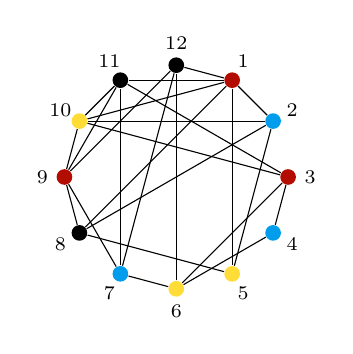
\begin{tikzpicture}
        \begin{scope}[every node/.style = {font=\scriptsize}]
        \newcount \myc
        \foreach \n in {1, 3, 9}{
            \myc=\n \advance\myc by -1 \multiply\myc by -360 \divide\myc by 12 \advance\myc by 60.0
            \node[anchor=center] (L\n) at (\the\myc:1.7) {\n};
            \node[anchor=center, circle, fill=uofgpillarbox, inner sep=2pt] (N\n) at (\the\myc:1.42) {};
        }
        \foreach \n in {2, 4, 7}{
            \myc=\n \advance\myc by -1 \multiply\myc by -360 \divide\myc by 12 \advance\myc by 60.0
            \node[anchor=center] (L\n) at (\the\myc:1.7) {\n};
            \node[anchor=center, circle, fill=uofgcobalt, inner sep=2pt] (N\n) at (\the\myc:1.42) {};
        }
        \foreach \n in {5, 6, 10}{
            \myc=\n \advance\myc by -1 \multiply\myc by -360 \divide\myc by 12 \advance\myc by 60.0
            \node[anchor=center] (L\n) at (\the\myc:1.7) {\n};
            \node[anchor=center, circle, fill=uofgsunshine, inner sep=2pt] (N\n) at (\the\myc:1.42) {};
        }
        \foreach \n in {8, 11, 12}{
            \myc=\n \advance\myc by -1 \multiply\myc by -360 \divide\myc by 12 \advance\myc by 60.0
            \node[anchor=center] (L\n) at (\the\myc:1.7) {\n};
            \node[anchor=center, circle, fill=black, inner sep=2pt] (N\n) at (\the\myc:1.42) {};
        }
        \draw (N1) -- (N2);
        \draw (N1) -- (N5);
        \draw (N1) -- (N8);
        \draw (N1) -- (N10);
        \draw (N1) -- (N11);
        \draw (N1) -- (N12);
        \draw (N2) -- (N5);
        \draw (N2) -- (N8);
        \draw (N2) -- (N10);
        \draw (N3) -- (N4);
        \draw (N3) -- (N6);
        \draw (N3) -- (N10);
        \draw (N3) -- (N11);
        \draw (N4) -- (N6);
        \draw (N5) -- (N8);
        \draw (N6) -- (N7);
        \draw (N6) -- (N12);
        \draw (N7) -- (N9);
        \draw (N7) -- (N11);
        \draw (N7) -- (N12);
        \draw (N8) -- (N9);
        \draw (N9) -- (N10);
        \draw (N9) -- (N11);
        \draw (N9) -- (N12);
        \draw (N10) -- (N11);
    \end{scope}
    \end{tikzpicture}\end{center}

    Given a $k$-colouring of a subgraph, that subgraph cannot have a clique of more than
    $k$ vertices.
    \begin{itemize}
        \item Each colour class describes an at-most-one constraint.
    \end{itemize}
    \colorred{This does \emph{not} follow 
%       from 
    by
    reverse unit propagation.}
\end{frame}

\begin{frame}{Recovering At-Most-One Constraints}
%       Can't list  %%% Just a suggestion -JN
    Practically infeasible to list
    every colour class we \emph{might} use in the pseudo-Boolean input.
    \\ \medskip
    But  %% -JN
    we can use cutting planes to recover colour classes lazily!
    \uncover<2->{
    \begin{align*}
        (\overline{x}_1 + \overline{x}_6 \ge 1)
%   \,\times\,2 
&
%    &=~& 
%   2\overline{x}_1 + 2\overline{x}_6 \ge 2 
\\
        +\,(\overline{x}_1 + \overline{x}_9 \ge 1) & &=~& 
2 \overline{x}_1 + 
\hphantom{2} \overline{x}_6 +
\hphantom{2} \overline{x}_9 
\ge 2 \\
        +\,(\overline{x}_6 + \overline{x}_9 \ge 1) & &=~& 
2 \overline{x}_1 + 
2 \overline{x}_6 + 
2 \overline{x}_9 
\ge 3 \\
%           /\,3 
        /\,2 
& &=~& 
\hphantom{2} \overline{x}_1 + 
\hphantom{2} \overline{x}_6 + 
\hphantom{2} \overline{x}_9 
\ge 2 \\
 && \text{i.e.}~ & x_1 + x_6 + x_9 \le 1
    \end{align*}}
    \uncover<3->{
    This generalises for arbitrarily large colour classes.
    \begin{itemize}
        \item Each non-edge is used exactly once, $v (v - 1)$ additions.
        \item 
%             $v - 2$ multiplications and divisions.
          $v - 3$ multiplications and $v-2$ divisions.
    \end{itemize}
    Solvers don't need to ``understand'' cutting planes to write this out.}
\end{frame}

\begin{nearlyplainframe}[t]{What This Looks Like}
\VerbatimInput[fontsize=\tiny,commandchars=\\\{\},codes={\catcode`$=3\catcode`^=7\catcode`_=8}]{clique-proof.veripb}
\end{nearlyplainframe}

\begin{frame}[fragile,t]{Verifying This Proof (For Real, This Time)}
\tiny%
\begin{Verbatim}[commandchars=\\\{\}]
$ veripb --trace clique.opb clique-attempt-two.veripb
=== begin trace ===
line 002: f 41
  ConstraintId \veripbid{001}: \veripbConstraint{1 ~x1 1 ~x3 >= 1}
  ConstraintId \veripbid{002}: \veripbConstraint{1 ~x2 1 ~x3 >= 1}
...
  ConstraintId \veripbid{041}: \veripbConstraint{1 ~x11 1 ~x12 >= 1}
line 003: o x7 x9 x12 ~x1 ~x2 ~x3 ~x4 ~x5 ~x6 ~x8 ~x10 ~x11
  ConstraintId \veripbid{042}: \veripbConstraint{1 x1 1 x2 1 x3 1 x4 1 x5 1 x6 1 x7 1 x8 1 x9 1 x10 1 x11 1 x12 >= 4}
line 004: u 1 ~x12 1 ~x7 >= 1 ;
  ConstraintId \veripbid{043}: \veripbConstraint{1 ~x7 1 ~x12 >= 1}
line 005: * bound, colour classes [ x1 x6 x9 ]
line 006: p 7 19 + 24 + 2 d
  ConstraintId \veripbid{044}: \veripbConstraint{1 ~x1 1 ~x6 1 ~x9 >= 2}
line 007: p 42 43 +
  ConstraintId \veripbid{045}: \veripbConstraint{1 x1 1 x2 1 x3 1 x4 1 x5 1 x6 1 x8 1 x9 1 x10 1 x11 >= 3}
...
  ConstraintId \veripbid{061}: \veripbConstraint{1 ~x5 1 ~x6 1 ~x10 >= 2}
line 028: p 53 57 + 59 + 61 +
  ConstraintId \veripbid{062}: \veripbConstraint{1 x8 1 x11 1 x12 >= 2}
line 029: u >= 1 ;
  ConstraintId \veripbid{063}: \veripbConstraint{>= 1}
line 030: c -1
=== end trace ===

Verification succeeded.
\end{Verbatim}
\end{frame}

\begin{frame}{Different Clique Algorithms}
  Different search orders? 
  \begin{itemize}
  \item[\checkmark] Irrelevant for proof logging.
  \end{itemize}
  \medskip
  Using local search to initialise?
  \begin{itemize}
  \item[\checkmark] 
    Just log the incumbent.
  \end{itemize}
  \medskip
  Different bound functions?
  \begin{itemize}
  \item Is cutting planes strong enough to
    justify every useful bound function ever invented?
  \item
    So far, seems like it\ldots
  \end{itemize}
  \medskip
  Weighted cliques?
  \begin{itemize}
  \item[\checkmark] Multiply a colour class by its largest weight.
  \item[\checkmark] Also works for vertices ``split between colour classes''.
  \end{itemize}
\end{frame}

\begin{frame}[t]{What About Subgraph Isomorphism?}
Each pattern vertex gets a target vertex: \begin{align*}
    \sum_{t \in \vertexset(T)} x_{p{,}t}  & = 1 && p \in \vertexset(P)
\end{align*}\pause
Each target vertex may be used at most once:\begin{align*}
    \sum_{p \in \vertexset(P)} -x_{p{,}t} & \ge -1 && t \in \vertexset(T)
\end{align*}\pause
Adjacency constraints, if $p$ is mapped to $t$, then $p$'s neighbours must
be mapped to $t$'s neighbours: \begin{align*}
    \overline{x}_{p{,}t} + \sum_{u \in \neighbourhood(t)} x_{q{,}u} & \ge 1 && p \in \vertexset(P),~q \in \neighbourhood(p),~t \in \vertexset(T)
\end{align*}
\end{frame}

\begin{frame}[fragile]{Degree Reasoning in Cutting Planes}
A pattern vertex $p$ of degree $\degree(p)$ can never be mapped to a target vertex $t$ of degree
$\degree(p)-1$ or lower in any subgraph isomorphism. \\
\medskip
    Observe $\neighbourhood(\textcolor{uofgcobalt}{p}) = \{ \textcolor{uofglawn}{q}, \textcolor{uofglawn}{r}, \textcolor{uofglawn}{s} \}$ and $\neighbourhood(\textcolor{uofgcobalt}{t}) = \{ \textcolor{uofgthistle}{u}, \textcolor{uofgthistle}{v} \}$.\\
\medskip
    We wish to derive $\overline{x}_{\textcolor{uofgcobalt}{p}{,}\textcolor{uofgcobalt}{t}} \ge 1$.
\begin{tikzpicture}[overlay,remember picture]
    \node [anchor=center, text depth=0.5cm, xshift=3.8cm, yshift=2.3cm]
    at (current page.center) {
        \begin{minipage}[t]{0.3\paperwidth}\raggedright
            \begin{tikzpicture}
                \node [draw, circle, fill=white, inner sep=2.5pt, font=\scriptsize] (NO) at (0, 0.7) {\phantom{1}};
                \node [anchor=center, font=\scriptsize] at (NO) {o};
                \node [draw, circle, fill=uofgcobalt, inner sep=2.5pt, font=\scriptsize] (NP) at (0, 0) {\phantom{1}};
                \node [anchor=center, font=\scriptsize] at (NP) {p};
                \node [draw, circle, fill=uofglawn, inner sep=2.5pt, font=\scriptsize] (NQ) at (0.7, 0.7) {\phantom{1}};
                \node [anchor=center, font=\scriptsize] at (NQ) {q};
                \node [draw, circle, fill=uofglawn, inner sep=2.5pt, font=\scriptsize] (NR) at (0.7, 0) {\phantom{1}};
                \node [anchor=center, font=\scriptsize] at (NR) {r};
                \node [draw, circle, fill=uofglawn, inner sep=2.5pt, font=\scriptsize] (NS) at (0.7, -0.7) {\phantom{1}};
                \node [anchor=center, font=\scriptsize] at (NS) {s};
                \draw (NO) -- (NQ);
                \draw (NP) -- (NQ);
                \draw (NP) -- (NR);
                \draw (NP) -- (NS);
                \draw (NQ) -- (NR);
                \draw (NR) -- (NS);

                \node [draw, circle, fill=uofgcobalt, inner sep=2.5pt, font=\scriptsize] (NT) at (1.75, 0) {\phantom{1}};
                \node [anchor=center, font=\scriptsize] at (NT) {t};
                \node [draw, circle, fill=uofgthistle, inner sep=2.5pt, font=\scriptsize] (NU) at (2.45, 0.7) {\phantom{1}};
                \node [anchor=center, font=\scriptsize] at (NU) {u};
                \node [draw, circle, fill=uofgthistle, inner sep=2.5pt, font=\scriptsize] (NV) at (2.45, 0) {\phantom{1}};
                \node [anchor=center, font=\scriptsize] at (NV) {v};
                \node [draw, circle, fill=white, inner sep=2.5pt, font=\scriptsize] (NX) at (3.15, 0.7) {\phantom{1}};
                \node [anchor=center, font=\scriptsize] at (NX) {x};
                \node [draw, circle, fill=white, inner sep=2.5pt, font=\scriptsize] (NY) at (3.15, 0) {\phantom{1}};
                \node [anchor=center, font=\scriptsize] at (NY) {y};
                \node [draw, circle, fill=white, inner sep=2.5pt, font=\scriptsize] (NZ) at (3.15, -0.7) {\phantom{1}};
                \node [anchor=center, font=\scriptsize] at (NZ) {z};
                \draw (NT) -- (NU);
                \draw (NT) -- (NV);
                \draw (NU) -- (NV);
                \draw (NU) -- (NX);
                \draw (NU) -- (NY);
                \draw (NV) -- (NY);
                \draw (NX) -- (NY);
                \draw (NY) -- (NZ);
                \draw (NV) -- (NZ);
            \end{tikzpicture}
        \end{minipage}
    };
\end{tikzpicture}
\end{frame}

\begin{frame}[fragile]{Degree Reasoning in Cutting Planes}
    We have the three adjacency constraints,
\begin{align*}
    \overline{x}_{\textcolor{uofgcobalt}{p}{,}\textcolor{uofgcobalt}{t}} + x_{\textcolor{uofglawn}{q}{,}\textcolor{uofgthistle}{u}} + x_{\textcolor{uofglawn}{q}{,}\textcolor{uofgthistle}{v}} & \ge 1 \\
    \overline{x}_{\textcolor{uofgcobalt}{p}{,}\textcolor{uofgcobalt}{t}} + x_{\textcolor{uofglawn}{r}{,}\textcolor{uofgthistle}{u}} + x_{\textcolor{uofglawn}{r}{,}\textcolor{uofgthistle}{v}} & \ge 1 \\
    \overline{x}_{\textcolor{uofgcobalt}{p}{,}\textcolor{uofgcobalt}{t}} + x_{\textcolor{uofglawn}{s}{,}\textcolor{uofgthistle}{u}} + x_{\textcolor{uofglawn}{s}{,}\textcolor{uofgthistle}{v}} & \ge 1
\end{align*}
Their sum is
\begin{align*}
    3 \overline{x}_{\textcolor{uofgcobalt}{p}{,}\textcolor{uofgcobalt}{t}} + x_{\textcolor{uofglawn}{q}{,}\textcolor{uofgthistle}{u}} + x_{\textcolor{uofglawn}{q}{,}\textcolor{uofgthistle}{v}}
    + x_{\textcolor{uofglawn}{r}{,}\textcolor{uofgthistle}{u}} + x_{\textcolor{uofglawn}{r}{,}\textcolor{uofgthistle}{v}}
    + x_{\textcolor{uofglawn}{s}{,}\textcolor{uofgthistle}{u}} + x_{\textcolor{uofglawn}{s}{,}\textcolor{uofgthistle}{v}} & \ge 3
\end{align*}
\begin{tikzpicture}[overlay,remember picture]
    \node [anchor=center, text depth=0.5cm, xshift=3.8cm, yshift=2.3cm]
    at (current page.center) {
        \begin{minipage}[t]{0.3\paperwidth}\raggedright
            \begin{tikzpicture}
                \node [draw, circle, fill=white, inner sep=2.5pt, font=\scriptsize] (NO) at (0, 0.7) {\phantom{1}};
                \node [anchor=center, font=\scriptsize] at (NO) {o};
                \node [draw, circle, fill=uofgcobalt, inner sep=2.5pt, font=\scriptsize] (NP) at (0, 0) {\phantom{1}};
                \node [anchor=center, font=\scriptsize] at (NP) {p};
                \node [draw, circle, fill=uofglawn, inner sep=2.5pt, font=\scriptsize] (NQ) at (0.7, 0.7) {\phantom{1}};
                \node [anchor=center, font=\scriptsize] at (NQ) {q};
                \node [draw, circle, fill=uofglawn, inner sep=2.5pt, font=\scriptsize] (NR) at (0.7, 0) {\phantom{1}};
                \node [anchor=center, font=\scriptsize] at (NR) {r};
                \node [draw, circle, fill=uofglawn, inner sep=2.5pt, font=\scriptsize] (NS) at (0.7, -0.7) {\phantom{1}};
                \node [anchor=center, font=\scriptsize] at (NS) {s};
                \draw (NO) -- (NQ);
                \draw (NP) -- (NQ);
                \draw (NP) -- (NR);
                \draw (NP) -- (NS);
                \draw (NQ) -- (NR);
                \draw (NR) -- (NS);

                \node [draw, circle, fill=uofgcobalt, inner sep=2.5pt, font=\scriptsize] (NT) at (1.75, 0) {\phantom{1}};
                \node [anchor=center, font=\scriptsize] at (NT) {t};
                \node [draw, circle, fill=uofgthistle, inner sep=2.5pt, font=\scriptsize] (NU) at (2.45, 0.7) {\phantom{1}};
                \node [anchor=center, font=\scriptsize] at (NU) {u};
                \node [draw, circle, fill=uofgthistle, inner sep=2.5pt, font=\scriptsize] (NV) at (2.45, 0) {\phantom{1}};
                \node [anchor=center, font=\scriptsize] at (NV) {v};
                \node [draw, circle, fill=white, inner sep=2.5pt, font=\scriptsize] (NX) at (3.15, 0.7) {\phantom{1}};
                \node [anchor=center, font=\scriptsize] at (NX) {x};
                \node [draw, circle, fill=white, inner sep=2.5pt, font=\scriptsize] (NY) at (3.15, 0) {\phantom{1}};
                \node [anchor=center, font=\scriptsize] at (NY) {y};
                \node [draw, circle, fill=white, inner sep=2.5pt, font=\scriptsize] (NZ) at (3.15, -0.7) {\phantom{1}};
                \node [anchor=center, font=\scriptsize] at (NZ) {z};
                \draw (NT) -- (NU);
                \draw (NT) -- (NV);
                \draw (NU) -- (NV);
                \draw (NU) -- (NX);
                \draw (NU) -- (NY);
                \draw (NV) -- (NY);
                \draw (NX) -- (NY);
                \draw (NY) -- (NZ);
                \draw (NV) -- (NZ);
            \end{tikzpicture}
        \end{minipage}
    };
\end{tikzpicture}
\end{frame}

\begin{frame}[fragile]{Degree Reasoning in Cutting Planes}
Continuing with the sum
\begin{align*}
    3 \overline{x}_{\textcolor{uofgcobalt}{p}{,}\textcolor{uofgcobalt}{t}} + x_{\textcolor{uofglawn}{q}{,}\textcolor{uofgthistle}{u}} + x_{\textcolor{uofglawn}{q}{,}\textcolor{uofgthistle}{v}}
    + x_{\textcolor{uofglawn}{r}{,}\textcolor{uofgthistle}{u}} + x_{\textcolor{uofglawn}{r}{,}\textcolor{uofgthistle}{v}}
    + x_{\textcolor{uofglawn}{s}{,}\textcolor{uofgthistle}{u}} + x_{\textcolor{uofglawn}{s}{,}\textcolor{uofgthistle}{v}} & \ge 3
\end{align*}
    Due to injectivity,\begin{align*}
        &-x_{o{,}\textcolor{uofgthistle}{u}} + -x_{\textcolor{uofgcobalt}{p}{,}\textcolor{uofgthistle}{u}} + -x_{\textcolor{uofglawn}{q}{,}\textcolor{uofgthistle}{u}} + -x_{\textcolor{uofglawn}{r}{,}\textcolor{uofgthistle}{u}} + -x_{\textcolor{uofglawn}{s}{,}\textcolor{uofgthistle}{u}} \ge -1 \\
        &-x_{o{,}\textcolor{uofgthistle}{v}} + -x_{\textcolor{uofgcobalt}{p}{,}\textcolor{uofgthistle}{v}} + -x_{\textcolor{uofglawn}{q}{,}\textcolor{uofgthistle}{v}} + -x_{\textcolor{uofglawn}{r}{,}\textcolor{uofgthistle}{v}} + -x_{\textcolor{uofglawn}{s}{,}\textcolor{uofgthistle}{v}} \ge -1
    \end{align*}
    Add all these together, getting \[
        3 \overline{x}_{\textcolor{uofgcobalt}{p}{,}\textcolor{uofgcobalt}{t}} + -x_{o{,}\textcolor{uofgthistle}{u}} + -x_{o{,}\textcolor{uofgthistle}{v}} + -x_{\textcolor{uofgcobalt}{p}{,}\textcolor{uofgthistle}{u}} + -x_{\textcolor{uofgcobalt}{p}{,}\textcolor{uofgthistle}{v}} \ge 1\]
\begin{tikzpicture}[overlay,remember picture]
    \node [anchor=center, text depth=0.5cm, xshift=3.8cm, yshift=2.3cm]
    at (current page.center) {
        \begin{minipage}[t]{0.3\paperwidth}\raggedright
            \begin{tikzpicture}
                \node [draw, circle, fill=white, inner sep=2.5pt, font=\scriptsize] (NO) at (0, 0.7) {\phantom{1}};
                \node [anchor=center, font=\scriptsize] at (NO) {o};
                \node [draw, circle, fill=uofgcobalt, inner sep=2.5pt, font=\scriptsize] (NP) at (0, 0) {\phantom{1}};
                \node [anchor=center, font=\scriptsize] at (NP) {p};
                \node [draw, circle, fill=uofglawn, inner sep=2.5pt, font=\scriptsize] (NQ) at (0.7, 0.7) {\phantom{1}};
                \node [anchor=center, font=\scriptsize] at (NQ) {q};
                \node [draw, circle, fill=uofglawn, inner sep=2.5pt, font=\scriptsize] (NR) at (0.7, 0) {\phantom{1}};
                \node [anchor=center, font=\scriptsize] at (NR) {r};
                \node [draw, circle, fill=uofglawn, inner sep=2.5pt, font=\scriptsize] (NS) at (0.7, -0.7) {\phantom{1}};
                \node [anchor=center, font=\scriptsize] at (NS) {s};
                \draw (NO) -- (NQ);
                \draw (NP) -- (NQ);
                \draw (NP) -- (NR);
                \draw (NP) -- (NS);
                \draw (NQ) -- (NR);
                \draw (NR) -- (NS);

                \node [draw, circle, fill=uofgcobalt, inner sep=2.5pt, font=\scriptsize] (NT) at (1.75, 0) {\phantom{1}};
                \node [anchor=center, font=\scriptsize] at (NT) {t};
                \node [draw, circle, fill=uofgthistle, inner sep=2.5pt, font=\scriptsize] (NU) at (2.45, 0.7) {\phantom{1}};
                \node [anchor=center, font=\scriptsize] at (NU) {u};
                \node [draw, circle, fill=uofgthistle, inner sep=2.5pt, font=\scriptsize] (NV) at (2.45, 0) {\phantom{1}};
                \node [anchor=center, font=\scriptsize] at (NV) {v};
                \node [draw, circle, fill=white, inner sep=2.5pt, font=\scriptsize] (NX) at (3.15, 0.7) {\phantom{1}};
                \node [anchor=center, font=\scriptsize] at (NX) {x};
                \node [draw, circle, fill=white, inner sep=2.5pt, font=\scriptsize] (NY) at (3.15, 0) {\phantom{1}};
                \node [anchor=center, font=\scriptsize] at (NY) {y};
                \node [draw, circle, fill=white, inner sep=2.5pt, font=\scriptsize] (NZ) at (3.15, -0.7) {\phantom{1}};
                \node [anchor=center, font=\scriptsize] at (NZ) {z};
                \draw (NT) -- (NU);
                \draw (NT) -- (NV);
                \draw (NU) -- (NV);
                \draw (NU) -- (NX);
                \draw (NU) -- (NY);
                \draw (NV) -- (NY);
                \draw (NX) -- (NY);
                \draw (NY) -- (NZ);
                \draw (NV) -- (NZ);
            \end{tikzpicture}
        \end{minipage}
    };
\end{tikzpicture}
\end{frame}

\begin{frame}[fragile]{Degree Reasoning in Cutting Planes}
    We're more or less there. We have: \[
        3 \overline{x}_{\textcolor{uofgcobalt}{p}{,}\textcolor{uofgcobalt}{t}} + -x_{o{,}\textcolor{uofgthistle}{u}} + -x_{o{,}\textcolor{uofgthistle}{v}} + -x_{\textcolor{uofgcobalt}{p}{,}\textcolor{uofgthistle}{u}} + -x_{\textcolor{uofgcobalt}{p}{,}\textcolor{uofgthistle}{v}} \ge 1\]

    Add the literal axioms $x_{o{,}\textcolor{uofgthistle}{u}} \ge 0$, $x_{o{,}\textcolor{uofgthistle}{v}} \ge 0$, $x_{\textcolor{uofgcobalt}{p}{,}\textcolor{uofgthistle}{u}} \ge 0$ and $x_{\textcolor{uofgcobalt}{p}{,}\textcolor{uofgthistle}{v}} \ge 0$ to get \[
        3 \overline{x}_{\textcolor{uofgcobalt}{p}{,}\textcolor{uofgcobalt}{t}} \ge 1\]
Divide by 3 to get the desired \[
    \overline{x}_{\textcolor{uofgcobalt}{p}{,}\textcolor{uofgcobalt}{t}} \ge 1\]
\begin{tikzpicture}[overlay,remember picture]
    \node [anchor=center, text depth=0.5cm, xshift=3.8cm, yshift=2.3cm]
    at (current page.center) {
        \begin{minipage}[t]{0.3\paperwidth}\raggedright
            \begin{tikzpicture}
                \node [draw, circle, fill=white, inner sep=2.5pt, font=\scriptsize] (NO) at (0, 0.7) {\phantom{1}};
                \node [anchor=center, font=\scriptsize] at (NO) {o};
                \node [draw, circle, fill=uofgcobalt, inner sep=2.5pt, font=\scriptsize] (NP) at (0, 0) {\phantom{1}};
                \node [anchor=center, font=\scriptsize] at (NP) {p};
                \node [draw, circle, fill=uofglawn, inner sep=2.5pt, font=\scriptsize] (NQ) at (0.7, 0.7) {\phantom{1}};
                \node [anchor=center, font=\scriptsize] at (NQ) {q};
                \node [draw, circle, fill=uofglawn, inner sep=2.5pt, font=\scriptsize] (NR) at (0.7, 0) {\phantom{1}};
                \node [anchor=center, font=\scriptsize] at (NR) {r};
                \node [draw, circle, fill=uofglawn, inner sep=2.5pt, font=\scriptsize] (NS) at (0.7, -0.7) {\phantom{1}};
                \node [anchor=center, font=\scriptsize] at (NS) {s};
                \draw (NO) -- (NQ);
                \draw (NP) -- (NQ);
                \draw (NP) -- (NR);
                \draw (NP) -- (NS);
                \draw (NQ) -- (NR);
                \draw (NR) -- (NS);

                \node [draw, circle, fill=uofgcobalt, inner sep=2.5pt, font=\scriptsize] (NT) at (1.75, 0) {\phantom{1}};
                \node [anchor=center, font=\scriptsize] at (NT) {t};
                \node [draw, circle, fill=uofgthistle, inner sep=2.5pt, font=\scriptsize] (NU) at (2.45, 0.7) {\phantom{1}};
                \node [anchor=center, font=\scriptsize] at (NU) {u};
                \node [draw, circle, fill=uofgthistle, inner sep=2.5pt, font=\scriptsize] (NV) at (2.45, 0) {\phantom{1}};
                \node [anchor=center, font=\scriptsize] at (NV) {v};
                \node [draw, circle, fill=white, inner sep=2.5pt, font=\scriptsize] (NX) at (3.15, 0.7) {\phantom{1}};
                \node [anchor=center, font=\scriptsize] at (NX) {x};
                \node [draw, circle, fill=white, inner sep=2.5pt, font=\scriptsize] (NY) at (3.15, 0) {\phantom{1}};
                \node [anchor=center, font=\scriptsize] at (NY) {y};
                \node [draw, circle, fill=white, inner sep=2.5pt, font=\scriptsize] (NZ) at (3.15, -0.7) {\phantom{1}};
                \node [anchor=center, font=\scriptsize] at (NZ) {z};
                \draw (NT) -- (NU);
                \draw (NT) -- (NV);
                \draw (NU) -- (NV);
                \draw (NU) -- (NX);
                \draw (NU) -- (NY);
                \draw (NV) -- (NY);
                \draw (NX) -- (NY);
                \draw (NY) -- (NZ);
                \draw (NV) -- (NZ);
            \end{tikzpicture}
        \end{minipage}
    };
\end{tikzpicture}
\end{frame}

\begin{frame}[fragile]{Degree Reasoning in VeriPB}
\begin{Verbatim}[commandchars=\\\{\},codes={\catcode`$=3\catcode`^=7\catcode`_=8}]
p \textcolor{uofglawn}{18}$_{\textcolor{uofgheather}{p{\sim}t{:}q}}$ \textcolor{uofglawn}{19}$_{\textcolor{uofgheather}{p{\sim}t{:}r}}$ + \textcolor{uofglawn}{20}$_{\textcolor{uofgheather}{p{\sim}t{:}s}}$ +   \textcolor{uofgcobalt}{* sum adjacency constraints}
  \textcolor{uofglawn}{12}$_{\textcolor{uofgheather}{inj(u)}}$ + \textcolor{uofglawn}{13}$_{\textcolor{uofgheather}{inj(v)}}$ +        \,\,\textcolor{uofgcobalt}{* sum injectivity constraints}
  xo\textunderscore{}u + xo\textunderscore{}v +            \textcolor{uofgcobalt}{* cancel stray xo\textunderscore{}*}
  xp\textunderscore{}u + xp\textunderscore{}v +            \textcolor{uofgcobalt}{* cancel stray xp\textunderscore{}*}
  \textcolor{uofgpumpkin}{3} d                      \textcolor{uofgcobalt}{* divide, and we're done}
\end{Verbatim}

\medskip

Or we can ask VeriPB to do the last bit of simplification automatically:

\medskip

\begin{Verbatim}[commandchars=\\\{\},codes={\catcode`$=3\catcode`^=7\catcode`_=8}]
p \textcolor{uofglawn}{18}$_{\textcolor{uofgheather}{p{\sim}t{:}q}}$ \textcolor{uofglawn}{19}$_{\textcolor{uofgheather}{p{\sim}t{:}r}}$ + \textcolor{uofglawn}{20}$_{\textcolor{uofgheather}{p{\sim}t{:}s}}$ +   \textcolor{uofgcobalt}{* sum adjacency constraints}
  \textcolor{uofglawn}{12}$_{\textcolor{uofgheather}{inj(u)}}$ + \textcolor{uofglawn}{13}$_{\textcolor{uofgheather}{inj(v)}}$ +        \,\,\textcolor{uofgcobalt}{* sum injectivity constraints}
j \textcolor{uofgpillarbox}{-1} 1 ~xp\textunderscore{}t >= 1 ;        \textcolor{uofgcobalt}{* desired conclusion is implied}
\end{Verbatim}
%%% Just experimenting above, Ciaran --- feel free to change back -JN
%   * and simplify the above%
%
\end{frame}

\begin{frame}{Other Forms of Reasoning}
We can also log all of the other things state of the art subgraph solvers do:
\begin{itemize}
    \item Injectivity reasoning and filtering.
    \item Distance filtering.
    \item Neighbourhood degree sequences.
    \item Path filtering.
    \item Supplemental graphs.
\end{itemize}
    \medskip
\uncover<2->{
Proof steps are ``efficient'' using cutting planes.
    \begin{itemize}
        \item The length of the proof steps are no worse than the time complexity of the reasoning algorithms.
        \item Most proof steps require only trivial additional computations.
    \end{itemize}}
\end{frame}

\section{Stronger Proofs}

\begin{frame}{Extension Variables}
  Suppose we want new, fresh variable
  $a$ encoding
  \begin{equation*}
      \textcolor{uofglawn}{
        a 
        \lequiv 
        ( 3x + 2y + z + w \ge 3 )
%           (\varx \land y)
      }
  \end{equation*}

  Introduce constraints
  \begin{equation*}
      \textcolor{uofgcobalt}{
%           a \lor \olnot{\varx} \lor \olnot{y}
%       \qquad
    3 \olnot{a} + 3x + 2y + z + w \ge 3 
%       \olnot{a} \lor \varx
    \qquad
    5 a + 
    3 \olnot{x} + 2 \olnot{y}  + \olnot{z} + \olnot{w} \ge 5
%       \olnot{a} \lor y
}
  \end{equation*}

  Should be fine, so long as $a$ hasn't been used before.
\end{frame}

\begin{frame}{Symmetries}
    \begin{center}
    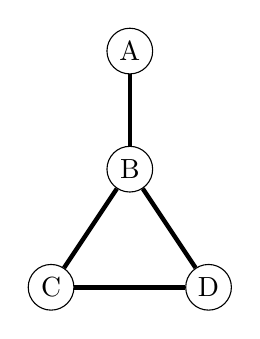
\begin{tikzpicture}
        \node <1> [draw, circle, fill=white, inner sep=4pt, font=\bfseries] (Na) at (1,  0) {\vphantom{1}};
        \node <1> [draw, circle, fill=white, inner sep=4pt, font=\bfseries] (Nb) at (1, -1.5) {\vphantom{1}};
        \node <1> [draw, circle, fill=white, inner sep=4pt, font=\bfseries] (Nc) at (0, -3) {\vphantom{1}};
        \node <1> [draw, circle, fill=white, inner sep=4pt, font=\bfseries] (Nd) at (2, -3) {\vphantom{1}};
        \node at (Na) {A};
        \node at (Nb) {B};
        \node at (Nc) {C};
        \node at (Nd) {D};

        \draw [ultra thick] (Na) -- (Nb);
        \draw [ultra thick] (Nb) -- (Nc);
        \draw [ultra thick] (Nc) -- (Nd);
        \draw [ultra thick] (Nb) -- (Nd);
    \end{tikzpicture}
    \end{center}

    \begin{itemize}
        \item If a solution exists, a solution where $C < D$ exists.
    \end{itemize}
\end{frame}

\begin{frame}{Dominance}
    \begin{center}\vspace*{-1em}
    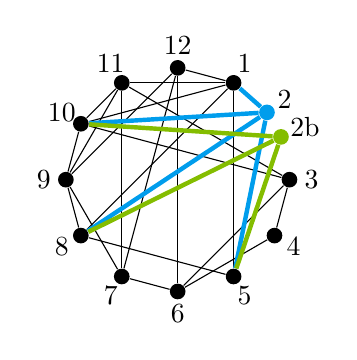
\begin{tikzpicture}
        \begin{scope}[scale=1]
        \newcount \myc
        \foreach \n in {1, 3, 4, 5, 6, 7, 8, 9, 10, 11, 12}{
            \myc=\n \advance\myc by -1 \multiply\myc by -360 \divide\myc by 12 \advance\myc by 60.0
            \node[anchor=center] (L\n) at (\the\myc:1.7) {\n};
            \node[anchor=center, circle, fill=black, inner sep=2pt] (N\n) at (\the\myc:1.42) {};
        }
        \foreach \n in {2}{
            \myc=\n \advance\myc by -1 \multiply\myc by -360 \divide\myc by 12 \advance\myc by 67.5
            \node[anchor=center] (L\n) at (\the\myc:1.7) {\n};
            \node[anchor=center, circle, fill=uofgcobalt, inner sep=2pt] (N\n) at (\the\myc:1.42) {};
        }
            \node[anchor=center] (L2b) at (22.5:1.75) {2b};
            \node[anchor=center, circle, fill=uofglawn, inner sep=2pt] (N2b) at (22.5:1.42) {};
        \draw <1> (N1) -- (N5);
        \draw <1> (N1) -- (N8);
        \draw (N1) -- (N10);
        \draw (N1) -- (N11);
        \draw (N1) -- (N12);
        \draw (N3) -- (N4);
        \draw (N3) -- (N6);
        \draw (N3) -- (N10);
        \draw (N3) -- (N11);
        \draw (N4) -- (N6);
        \draw <1> (N5) -- (N8);
        \draw (N6) -- (N7);
        \draw (N6) -- (N12);
        \draw (N7) -- (N9);
        \draw (N7) -- (N11);
        \draw (N7) -- (N12);
        \draw (N8) -- (N9);
        \draw (N9) -- (N10);
        \draw (N9) -- (N11);
        \draw (N9) -- (N12);
        \draw (N10) -- (N11);
            \draw [ultra thick, color=uofgcobalt] (N1) -- (N2);
            \draw [ultra thick, color=uofgcobalt] (N2) -- (N5);
            \draw [ultra thick, color=uofgcobalt] (N2) -- (N8);
            \draw [ultra thick, color=uofgcobalt] (N2) -- (N10);
            \draw [ultra thick, color=uofglawn] (N2b) -- (N5);
            \draw [ultra thick, color=uofglawn] (N2b) -- (N8);
            \draw [ultra thick, color=uofglawn] (N2b) -- (N10);
    \end{scope}
    \end{tikzpicture}
\end{center}
\medskip
    Can ignore vertex 2b.
    \begin{itemize}\item Every neighbour of 2b is also a neighbour of 2.
    \end{itemize}
\end{frame}


\section{Challenges}

\begin{frame}{Progress So Far on World Domination}
    \begin{itemize}
        \item SAT with symmetries, cardinality, XOR reasoning, MaxSAT.
            \begin{itemize}
                \item Uncovered several undetected bugs in state of the art solvers.
                \item Can't do MaxSAT hitting set solvers yet, MIP isn't proof logged.
            \end{itemize}
        \item Certified translations from pseudo-Boolean to CNF.
        \item Clique, subgraph isomorphism, maximum common (connected) induced subgraph.
        \item Constraint programming.
            \begin{itemize}
                \item Large integer variables.
                \item Absolute value, all different, circuit, comparison, element, linear equality
                    and inequality, minimum and maximum, regular, smart table constraints.
            \end{itemize}
        \item In progress: MIP preprocessing for pseudo-Boolean problems, dynamic programming,
             the remaining 400 constraints for CP, \ldots
    \end{itemize}
\end{frame}

\begin{frame}{What Reasoning Can We Justify?}
    \begin{itemize}
        \item With extension variables, as strong as Extended Frege.
        \item So according to theorists, we can simulate pretty much everything.
            \begin{itemize}
                \item <2-> Up to a polynomial factor\ldots
            \end{itemize}
        \item <3-> Dominance is apparently even stronger.
    \end{itemize}
\end{frame}

\begin{frame}{What Reasoning Can We Justify Efficiently?}
    \begin{itemize}
        \item Quadratic overheads are unpleasant.
        \item Cutting planes is very good at justifying combinatorial arguments.
        \item It's not really clear why.
    \end{itemize}
\end{frame}

\begin{frame}{Verifying the Verifier}
    \begin{itemize}
        \item How do we know the encoding is correct?
        \item How do we know the verifier is correct?
        \item How do we know the proof system is sound?
    \end{itemize}
\end{frame}

\begin{frame}{Proof Trimming}
    \begin{itemize}
        \item Proofs can be really really really big.
        \item Often many steps end up being redundant for the final proof.
        \item Could we make a tool that turns a really really really big proof into a really big
            proof?
    \end{itemize}
\end{frame}

\begin{frame}{Counting and Sampling without Enumerating}
    \begin{itemize}
        \item The proof system deals with unsatisfiability.
        \item Satisfiability is easy, just give a solution.
        \item Optimisation is a solution and a proof there's nothing better.
        \item Enumeration is a solution list, and a proof there's nothing else.
        \item How do we provide a count without enumerating?
    \end{itemize}
\end{frame}

\begin{frame}{Going the Other Way}
    \begin{itemize}
        \item Can we use proofs to understand solver behaviour?
            \begin{itemize}
                \item Why solvers work so well when they shouldn't.
                \item Why solvers perform so badly when they shouldn't.
            \end{itemize}
        \item Explainability?
    \end{itemize}
\end{frame}

\section{Propaganda}

\begin{frame}{Where We're At}
    \begin{itemize}
        \item Can verify \emph{solutions} from state of the art combinatorial solving algorithms,
            in a unified proof system.
        \item Found many undetected bugs in widely used solvers.
            \begin{itemize}
                \item Including in algorithms that have been ``proved'' correct.
            \end{itemize}
        \item <2-> Not being either proof logged or formally verified should be considered socially
            unacceptable.
        \item <3-> Perhaps studying proof logs can help explain why solvers work so well?
    \end{itemize}
\end{frame}

\begin{frame}{Getting Involved}
    \begin{center}
        \url{https://gitlab.com/MIAOresearch/software/VeriPB} \\
        \bigskip
        \url{https://satcompetition.github.io/2023/downloads/proposals/veripb.pdf} \\
        \bigskip
        \url{https://www.youtube.com/watch?v=s_5BIi4I22w} \\
        \bigskip
    \end{center}
\end{frame}

{
    \usebackgroundtemplate{
        \tikz[overlay, remember picture]
        \node[at=(current page.south), anchor=south, inner
        sep=0pt]{\includegraphics[keepaspectratio=true, width=\paperwidth]{../../images/background2.jpg}};
    }

    \begin{frame}[plain,noframenumbering]
        \begin{tikzpicture}[remember picture, overlay]
            \node at (current page.north west) {
                \begin{tikzpicture}[remember picture, overlay]
                    \fill [fill=uofguniversityblue, anchor=north west] (0, 0) rectangle (\paperwidth, -2.8cm);
                \end{tikzpicture}
            };

            \node (logo) [anchor=north east, shift={(-0.6cm,-0.2cm)}] at (current page.north east) {
                
\includegraphics[keepaspectratio=true,scale=0.5]{../../images/UoG_keyline.pdf}
            };

            \node (logo2) [anchor=north, below=0.2cm of logo.south] {
                
\includegraphics[keepaspectratio=true,scale=0.1]{../../images/RAEngWhite.pdf}
            };

            \coordinate (logos) at ($(logo.south)!0.5!(logo2.north)$);

            \node [anchor=west, xshift=0.2cm] at (current page.west |- logos) {
                \begin{minipage}{0.60\paperwidth}\raggedright
                    \textcolor{white}{\url{https://ciaranm.github.io/}} \\[0.3cm]
                    \textcolor{white}{\href{mailto:ciaran.mccreesh@glasgow.ac.uk}{\nolinkurl{ciaran.mccreesh@glasgow.ac.uk}}}
                \end{minipage}
            };
        \end{tikzpicture}
    \end{frame}
}

\end{document}

